\documentclass[a4paper,11pt,oneside]{article}
\usepackage[T1]{fontenc}
%----------------palatino fonts
\usepackage[sc,osf]{mathpazo}
\linespread{1.05}
%----------------hasta aqu\'i
\usepackage[utf8]{inputenc}
\usepackage[longnamesfirst,authoryear]{natbib}
\usepackage[table,xcdraw]{xcolor}
% \usepackage[spanish]{babel}
\usepackage{rotating}
\usepackage{epsfig}
%\usepackage{doublespace}
%\usepackage{endnotes}
%\usepackage{times}
\usepackage{longtable}
\usepackage{amsmath}
\usepackage{threeparttable}
\usepackage{amstext}
\usepackage{amssymb}
\usepackage{shadow}
\usepackage{soul}
\usepackage{ulem}
%--------------package para que ponga en negrita las letras griegas
\usepackage{amsbsy}
%--------------por desgracia, no lo hace. El que viene s\'i que lo hace, pero hay que dar la orden \bm{loqueseaparaponerloennegrita}
\usepackage{bm}
%\usepackage{mycaption}
\usepackage{psfrag}
%\usepackage{subfigure}
\usepackage{supertabular}
%--------------package para poner fusionar FILAS en una tabla----------
\usepackage{multirow}
%----------------Esto es lo que utilizo ahora de captions
\usepackage{hanging}
\usepackage[hang,normalsize,bf]{caption}
%\usepackage{hangcaption}
%-----------Este package que viene ahora hace que no corte cuando subrayamos. Para ello no podremos utilizar \underline{}, sino \emph{}
%-----------We will use soul instead of ulem:
\usepackage{soul}
%-----------Esto es lo que utilizaba antes-------------
%\usepackage[hang]{caption2}
\usepackage{sectsty}
%\usepackage{titlesec}
%\usepackage{hang}
%-----------Estos son paquetes que ha utilizado Ivan yo los incluyo pero no se muy bien como influiran---------------------
\usepackage{amsmath}
%\usepackage{chicago}
\usepackage{geometry}
\usepackage{setspace}
%-----------Para hacer que las filas de las tablas sean un poquito mas altas
\usepackage{array}
\usepackage{pdflscape}
\usepackage{graphicx}
\usepackage{tabularx}
\usepackage{color}
%\usepackage{eurosans,euro}
\usepackage{eurosym}
\usepackage{ntheorem}
\usepackage{booktabs}
%\usepackage{caption}
\usepackage{subcaption}
\usepackage{dcolumn}
\usepackage{booktabs}
\usepackage{float}
\usepackage{xr-hyper}
\usepackage{hyperref}
% \usepackage[style=authoryear,natbib=true,uniquename=init,firstinits,bibstyle=chicago]{biblatex}
%Package para las notas:
%\usepackage[colorinlistoftodos]{todonotes}
% \usepackage{tabular}

\usepackage{rotating}
%para rotar la tabla
\usepackage{appendix}
\usepackage{adjustbox}


\textwidth 162mm \textheight 236mm \topmargin -1.3cm
\oddsidemargin -0,1cm \pagestyle{plain}

%xr

% \externaldocument{Responses/response_rs_ref1}
% \externaldocument{Responses/response_rs_ref2}

%---acaba xr

%\newcommand{\thepagenumber}{--\arabic--}


% \definecolor{miguelangel}{rgb}{0.36,0.54,0.66}
% \newcommand{\Miguelangel}{\color{miguelangel}}

\definecolor{emili}{rgb}{0.47,0.27,0.23}
\newcommand{\Emili}{\color{emili}}

% \definecolor{luisa}{rgb}{0.97,0.17,0.93}
% \newcommand{\Luisa}{\color{luisa}}

%\definecolor{maite}{rgb}{0.37,0.47,0.13}
%\newcommand{\Maite}{\color{maite}}



% color rojo para los mensajes
\newcommand{\rojo}{\textcolor[rgb]{1.00,0.00,0.00}}

% color azul para los mensajes
\newcommand{\azul}{\textcolor[rgb]{0.00,0.00,1.00}}

% color verde para los mensajes
\newcommand{\verde}{\textcolor[rgb]{0.00,0.50,0.70}}

% color marron para los mensajes
\newcommand{\marron}{\textcolor[rgb]{0.80,0.50,0.00}}

\newcommand{\m}{Malmquist }

\newcommand{\mpi}{Malmquist productivity index }

\newcommand{\mpis}{Malmquist productivity indices }

\newcommand{\dos}{\renewcommand{\baselinestretch}{2}}
\renewcommand{\baselinestretch}{1.5}
\newcommand{\uno}{\renewcommand{\baselinestretch}{1}}

\renewcommand{\captionlabelfont}{\normalsize \bfseries}
\renewcommand{\captionfont}{\normalfont}

\newcommand\solidrule[1][1cm]{\rule[0.5ex]{#1}{.1pt}}
\newcommand\dashedrule{\mbox{%
  \solidrule[1mm]\hspace{.75mm}\solidrule[1mm]\hspace{.75mm}\solidrule[1mm]\hspace{.75mm}\solidrule[1mm]\hspace{.75mm}\solidrule[1mm]\hspace{.75mm}\solidrule[1mm]}}

\makeatletter
\def\@seccntformat#1{\csname the#1\endcsname.\quad}
\makeatother

%\sectionfont{\smallsize}

%\titleformat{\section}{\large\bfseries}{\thesection}{1em}{}


%\captionstyle{hang}

\sectionfont{\large\bf}
\subsectionfont{\normalsize\bf}


%\renewcommand{\footnote}{\endnote}


%\renewcommand{\tablename}{Cuadro}
%\renewcommand{\contentsname}{\'{I}ndice}
%\renewcommand{\figurename}{Gr\'{a}fico}
%\renewcommand{\listtablename}{\'{I}ndice de cuadros}
%\renewcommand{\listfigurename}{\'{I}ndice de gr\'{a}ficos}

%Este comando sirve para cambiar las fuentes de los entornos matem�ticos
%(definiciones, teoremas, etc.).
\theorembodyfont{\sl}

\theoremseparator{:}
\newtheorem{hyp}{Hypothesis}

\newtheorem{theorem}{Theorem}
\newtheorem{acknowledgement}{Acknowledgement}
\newtheorem{algorithm}{Algorithm}
\newtheorem{axiom}{Axiom}
\newtheorem{case}{Case}
\newtheorem{claim}{Claim}
\newtheorem{conclusion}{Conclusion}
\newtheorem{condition}{Condition}
\newtheorem{conjecture}{Conjecture}
\newtheorem{corollary}{Corollary}
\newtheorem{criterion}{Criterion}
\newtheorem{definition}{Definition}
%\newtheorem{definition}{Definition}
\newtheorem{example}{Example}
\newtheorem{exercise}{Exercise}
\newtheorem{lemma}{Lemma}
\newtheorem{notation}{Notation}
\newtheorem{problem}{Problem}
\newtheorem{proposition}{Proposition}
%\newtheorem{remark}{Remark}
\newtheorem{remark}{Nota}
\newtheorem{solution}{Solution}
\newtheorem{summary}{Summary}

\sloppy

\newenvironment{proof}[1][Proof]{\noindent\textbf{#1.} }{\ \rule{0.5em}{0.5em}}

%\geometry{left=0.90in,right=0.90in,top=0.50in,bottom=0.65in}

\renewcommand{\baselinestretch}{1.5}

\hyphenation{ma-kers}

%\hyphenation{pers-pec-ti-ve}
%\hyphenation{lear-ning}
%\hyphenation{im-pro-ving}
%\hyphenation{me-thods}
%\hyphenation{non-para-me-tric}
%\hyphenation{con-si-de-red}


\begin{document}


%\renewcommand{\tablename}{Cuadro}
%\renewcommand{\contentsname}{\'{I}ndice}
%\renewcommand{\figurename}{Gr\'{a}fico}
%\renewcommand{\listtablename}{\'{I}ndice de cuadros}
%\renewcommand{\listfigurename}{\'{I}ndice de gr\'{a}ficos}

%\begin{spacng}{1}






%\title{\textbf{Financial development traps and regional inequalities in Europe: Evidence from the financial sector}}

\title{\textbf{Financial Development Traps in European Regions: Theory and Evidence}\thanks{\color{black}All authors acknowledge financial support from MCIN/AEI/10.13039/501100011033 (Ministerio de Ciencia e Innovación, grants PID2019-109687GB-I00, PID2020-115450GB-I00, and PID2024-159788NB-I00). Emili Tortosa-Ausina also acknowledges support from the Generalitat Valenciana (CIPROM/2022/50). The usual disclaimer applies.}}



\author{\normalsize Rodrigo Cuenca De Armas \\ \textsl{\footnotesize Universitat Jaume I} \and \normalsize Maria Teresa Balaguer-Coll \\ \textsl{\footnotesize Universitat Jaume I} \and \normalsize Emili Tortosa-Ausina \\ \textsl{\footnotesize Universitat Jaume I, IIDL and Ivie}}



%\author{\textbf{\normalsize Authors?}}






%\date{March 2008}


%\bibliographystyle{normal3}

\bibliographystyle{apalike}


% \bibliographystyle{alphadin}

%\bibliographystyle{invest}

%\bibliographystyle{chicago}

\vspace{\stretch{1}}


\begin{spacing}{1}


\maketitle

\thispagestyle{empty}




\begin{abstract}


%ALTERNATIVE ABSTRACT:




%This study explores the risk of financial development traps in European regions by analyzing the performance of the financial sector in terms of productivity and employment, and its relationship with GDP per capita. Using data for 226 NUTS2 regions over the period 2000 to 2021, we construct two original indicators (FDTR1 and FDTR2) adapted from Diemer et al. (2022) to a sectoral framework. FDTR1 captures relative deceleration compared to past performance and EU benchmarks, while FDTR2 reflects structural slowdown. The analysis reveals that 8.2\% of the regions are trapped, with considerable heterogeneity between and within Eastern and Western Europe. Results show a reduction in the share of trapped regions between the 2008–2015 and 2016–2021 periods. Our findings highlight the importance of using both indicators in tandem and suggest that institutional and sectoral factors are likely to play a critical role in regional financial resilience beyond geographic location.

\textsl{This study explores the risk of financial development traps in European regions by analysing the performance of the financial sector in terms of productivity and its relationship with GDP per capita. Using data for 226 NUTS2 regions over the period 2000--2021, we construct two original indicators adapted from \cite{diemer2022regional} to a sectoral framework, capturing respectively the cyclical and structural dimensions of decoupling between financial sector dynamics and regional economic performance. The analysis reveals that a non-negligible share of European regions show signs of entrapment, with considerable heterogeneity both between and within Eastern and Western Europe. Results also point to a reduction in the share of trapped regions between the crisis period (2008--2015) and the subsequent recovery phase (2016--2021), alongside a notable inversion in the relative exposure of Eastern and Western European regions. Our findings highlight the importance of assessing the functional orientation of the financial sector (rather than its mere size or depth) and suggest that institutional and sectoral factors play a critical role in shaping regional financial resilience beyond geographic location.}






\end{abstract}



\vspace{0.6cm}

\noindent {\textbf{Key words and phrases}: financial development, development traps, regional inequalities, productivity, employment, convergence.}
\\

\noindent {\textbf{JEL Classifications}: R11, R58, O16, O18}
\\




\begin{sloppypar}
\noindent {\textbf{Communications to}: Emili Tortosa-Ausina, Departament d'Economia, Universitat Jaume I, Campus del Riu Sec, 12071 Castell\'o de la Plana, Spain. Tel.: +34 964387168, e-mail:} \texttt{tortosa@uji.es}.
\end{sloppypar}






\end{spacing}


\vspace*{\stretch{1}}



%\end{spacing}



\vspace*{\stretch{1}}



\pagebreak

%\tableofcontents

%\pagebreak

\setcounter{page}{1}



\section{Introduction}
\label{sec:intro}

%\Emili

In recent decades, the European Union has undergone profound transformations in its economic, social, and territorial structures \citep{bachtler2017eu,barbero2023improving}. Eastern enlargement, technological progress, and the consolidation of the single market have created new opportunities for growth, whilst simultaneously revealing persistent regional inequalities \citep{cappelen2003impact,iammarino2019regional}. Although many territories have converged towards income and welfare levels comparable to those of Europe's economic core, others have remained stagnant or experienced relative decline, failing to integrate fully into the dynamics of globalised growth. This situation has given rise to what the literature describes as a \textit{regional development trap}---a condition in which a region, despite having overcome underdevelopment, is no longer able to sustain convergence towards more advanced territories \citep{diemer2022regional}.


The persistence of such traps raises fundamental questions about the long-term sustainability of the European project. Regions that grow slowly and display signs of structural deceleration challenge the objective of territorial cohesion, a cornerstone of EU regional policy \citep{di2022one,caro2023role,rodriguez2025forging}. A growing body of research links these territorial dynamics to declining institutional trust and a weakening of the social fabric, particularly in regions that perceive themselves as left behind by national governments and European institutions \citep{rodriguez2018revenge,dijkstra2020geography,pike2024left,faggian2024three}. Beyond income dynamics, these processes point to persistent structural and institutional constraints that shape regional development paths over time.



Crucially, development traps are not necessarily the outcome of historical backwardness. In many cases, they emerge in regions that had previously improved their relative position but subsequently began to lose momentum. This loss of dynamism may take the form of deindustrialisation, outmigration of skilled workers, or stagnation in innovative capacity, generating self-reinforcing processes of decline \citep{cuadrado2016economic,iammarino2019regional}. Within the framework proposed by \cite{diemer2022regional}, these traps can be empirically identified through two complementary indicators, namely, DT1, which captures relative deterioration in growth dynamics, and DT2, which reflects persistent structural deceleration.



Although this framework has proven effective in identifying aggregate regional development traps, most existing applications rely on economy-wide indicators and devote limited attention to the role of specific sectors in shaping regional trajectories. Yet sectoral dynamics may prove decisive in determining whether regions sustain development momentum or drift into stagnation. Examining these dynamics therefore offers valuable insight into the mechanisms underlying heterogeneous regional outcomes.

%{\color{red} Why? Explanations.}



In our study, we apply the development-trap framework to a dataset of 226 European NUTS2 regions covering the period from 2000 to 2021, adopting a sectoral perspective that focuses on the financial sector rather than on the economy as a whole. Financial-sector performance is measured in terms of productivity and employment relative to the working-age population, whilst per capita GDP is included as an aggregate reference to link sectoral dynamics with broader patterns of economic development.


% {\color{red} Quizás Dariusz.}


Our approach offers a different perspective on the role of finance in regional development. Rather than assuming that the financial sector necessarily acts as a catalyst for economic convergence \citep{berthelemy1996economic,aghion2005effect}, it raises the question as to whether financial activity---despite its centrality in post-industrial economies---may instead contribute to spatial concentration, polarisation, and stagnation (even decline) in certain regions. By linking financial-sector productivity and employment dynamics with trajectories of per capita GDP, we aim to identify regions that exhibit signs of entering or consolidating a development trap, understood here as the inability to sustain financial-sector improvements that translate into long-term economic wellbeing \citep{wojcik2025finance}.

% {\color{red} (Meter aquí lo de Octavio, etc.; Lucio y Jaime EPA; why did cajas.)}

%To operationalise this approach, we replicate and adapt the set of indicators proposed by \cite{diemer2022regional}, conducting a regional analysis of growth accelerations and deviations relative to the European average. Unlike the original methodology, national-level comparisons are excluded; the indicators are therefore constructed using six components instead of nine, combining inter-temporal and European benchmarks for three key variables. The proposed indicators measure entrapment risk, whilst the subsequent classification defines trapped regions \textit{ex post}. Based on these measures, regions are classified as financially trapped, high-risk, or not trapped. We then examine the spatial distribution of these categories by distinguishing between Eastern and Western Europe and by providing some maps that allow visualising some of the identified patterns.



To operationalise this approach, we replicate and adapt the set of indicators proposed by \cite{diemer2022regional}, conducting a regional analysis of growth accelerations and deviations relative to the European average. Unlike the original methodology, national-level comparisons are excluded from the construction of the indicators. This decision is motivated by the sectoral and supranational focus of the study: since financial sector dynamics are shaped by European-level regulatory frameworks, monetary policy, and integration processes rather than exclusively by national economic conditions, benchmarking regions against the EU average might be more appropriate than benchmarking them against their respective national economies. Moreover, including national comparisons would risk convoluting the performance of the financial sector with broader country-level structural differences (such as institutional quality or fiscal capacity) that lie outside the scope of the present analysis. The indicators are therefore constructed using six components instead of nine, combining inter-temporal and European benchmarks for three key variables. The proposed indicators measure entrapment risk, whilst the subsequent classification defines trapped regions \textit{ex post}. Based on these measures, as we shall see, regions are classified as financially trapped, high-risk, or not trapped. We then examine the spatial distribution of these categories by distinguishing between Eastern and Western Europe and by providing some maps that allow visualising some of the identified patterns.



%Overall, our study contributes to ongoing debates on the role of strategic sectors in regional development by providing novel empirical evidence on the emergence of development traps within the financial sector---an increasingly influential domain in shaping Europe's contemporary economic geography and integration process.


Overall, our study contributes to ongoing debates on the role of strategic sectors in regional development \citep{balland2019smart} by providing novel empirical evidence on the emergence of development traps within the financial sector---an increasingly influential, albeit potentially destabilising, domain in shaping Europe's contemporary economic geography and integration process. A central theme running through our findings is that financial sector activity does not automatically translate into sustained regional economic improvements. Rather, in a substantial share of European regions, the financial sector appears to operate in a manner that is partly decoupled from the real economy: growing or restructuring in ways that fail to generate meaningful gains in employment, productivity, or per capita income for the broader regional population. This disconnection is not confined to economically lagging territories; it is also observable in wealthy Western European regions where sophisticated financial markets coexist with persistent structural misalignment between financial sector dynamics and regional development outcomes. By capturing both the cyclical and structural dimensions of this decoupling through the financial development trap indicators, our framework moves beyond conventional measures of financial depth or size, and instead assesses the functional capacity of the financial sector to contribute to regional prosperity---a distinction with direct implications for the design of cohesion policy and territorial development strategies across the European Union.




The remainder of the paper is organised as follows. Section~\ref{sec:background} reviews the theoretical foundations linking financial development and regional growth, with particular attention to convergence dynamics and development traps. Section~\ref{sec:methodology} presents the methodological framework and introduces the financial development trap indicators, whilst Section~\ref{sec:data} describes the data sources and sample composition. Section~\ref{sec:results} reports the empirical findings, highlighting substantial regional heterogeneity and East--West differences. Section~\ref{sec:discussion} discusses the results in relation to existing literature, focusing on mechanisms such as financial exclusion, institutional factors, and the financial curse phenomenon. Finally, Section~\ref{sec:conclusions} concludes and outlines policy implications and directions for future research.


\section{Related literature and background}
\label{sec:background}

\subsection{Financial development and its role in regional growth}


The relationship between financial development and economic growth has received a great deal of attention by the economics and finance literatures. Since the pioneering work of \cite{schumpeter.theory.1911}, there is a relatively wide consensus that a well-developed financial system can facilitate capital accumulation, mobilise savings, and finance innovation, which are key elements for sustaining long-term economic growth \citep{beck2000finance,demirguc2009finance}. This view has been reinforced by successive relevant contributions to the literature such as, for instance, \cite{levine2005finance}, who systematises the key functions of the financial system, including capital allocation, risk management, corporate control, and exchange facilitation, as mechanisms to drive growth.

%{\color{red} Se puede meter footnote de Robinson. Quizás mejor expandir por Robinson, incluso tema branches, y quitar el párrafo que sigue, que no pinta nada.}




%There are, however, different theoretical approaches to the functioning of the financial system. On the one hand, the \textit{bank-based view} emphasises the role of financial institutions as intermediaries that reduce information asymmetries and channel resources towards the most productive activities \citep{diamond1984financial,bencivenga1991financial}. On the other hand, the \textit{market-based view} stresses the importance of liquid and diversified financial markets as financing channels for innovative projects \citep{holmstrom1993market}. More recently, the \textit{functional view}, which focuses on the services provided by financial institutions beyond their organisational form, has gained prominence \citep{levine2002bank,bodie2005design}.


% At the regional level, financial development has been analysed as a possible explanatory factor for territorial divergences \citep{aghion2005effect,badunenko2013financial}. \cite{sokol2017financialisation} warns about the effects of the \textit{financial curse}, i.e. a process whereby the concentration of financial power in certain territories can exacerbate regional inequalities and weaken the links between finance and the real economy. In this regard, and in an study also applied to the European context, \cite{rossi2021financial} present a meta-analytical review that confirms a positive correlation between financial development and growth, albeit heterogeneous according to the institutional and geographical context.


At the regional level, financial development has been analysed as a possible explanatory factor for territorial divergence \citep{aghion2005effect,badunenko2013financial}. \cite{sokol2017financialisation} warns about the effects of the \textit{financial curse}, i.e. a process whereby the concentration of financial power in certain territories can exacerbate regional inequality and weaken the links between finance and the real economy. In this regard, \cite{rossi2021financial} provide empirical evidence for European regions showing that what drives regional economic growth is not the mere presence of banking services but rather the agglomeration of a complex and diversified financial sector---a finding that underscores the importance of the \textit{quality} and \textit{functional orientation} of financial activity, rather than its size or geographic diffusion. Crucially, their results also show that more financially developed regions are not necessarily more resilient to adverse economic shocks, a finding that resonates directly with our concern that financial sector activity may become structurally decoupled from regional development trajectories, giving rise to the entrapment dynamics we seek to identify.




% While the growth–finance nexus has been extensively documented at the national level, its regional manifestations remain more ambiguous \citep{dow1997regional}, as financial systems operate through spatially uneven institutional, sectoral, and organisational structures.


While the growth–finance nexus has been extensively documented at the national level, its regional manifestations remain less well understood \citep{wojcik2025finance}. As \cite{dow1997regional} emphasised in their survey of regional finance, financial systems do not operate uniformly across space: credit availability, liquidity preference, and the behaviour of financial intermediaries all vary systematically across regions, reflecting spatially uneven institutional, sectoral, and organisational structures. This spatial unevenness means that the relationship between financial development and regional economic performance cannot simply be inferred from national-level evidence---the same financial system may generate growth in some territories whilst constraining it in others. Such heterogeneity is precisely what the findings of \cite{rossi2021financial} and \cite{sokol2017financialisation} discussed above point to, and it provides the conceptual foundation for our approach: rather than assuming a uniform finance–growth relationship across European regions, we examine whether the financial sector generates the sort of productive, employment-supporting dynamics that translate into sustained regional development, or whether it becomes decoupled from the real economy in ways that contribute to entrapment.



\subsection{Regional convergence, territorial inequality and development traps}


The concept of a development trap refers to regions that face persistent difficulties in recovering past dynamism or improving the prosperity of their inhabitants \citep{diemer2022regional}. These territories have experienced a deterioration in economic growth, employment, and productivity relative to neighbouring regions and to their own historical trajectories. Such dynamics often generate social dissatisfaction and unrest, which, in the European context, have been closely associated with the rise of anti-system and Eurosceptic political movements \citep{dijkstra2020geography}.



% Although development traps are observed worldwide \citep{bonikowski2017ethno,rodrik2017populism}, the European case has been extensively documented. A broad literature highlights persistent territorial disparities in income levels, employment structures, business environment, education, productivity, and innovation capacity across European regions \citep{iammarino2019regional}. These imbalances have contributed to growing perceptions that existing economic systems no longer offer adequate protection or opportunities for large shares of the population.

Although development traps are observed across a wide range of economies and institutional contexts \citep{azariadis2005poverty,rodrik2016premature}, the European case has been extensively documented. A broad literature highlights persistent territorial disparities in income levels, employment structures, business environment, education, productivity, and innovation capacity across European regions \citep{iammarino2019regional,rodriguez2023left}. These imbalances have contributed to growing perceptions that existing economic systems no longer offer adequate protection or opportunities for large shares of the population \citep{bonikowski2017ethno,rodrik2017populism}.




%Traditionally, regional economic performance has been assessed using three core indicators: GDP per capita, employment, and productivity. Development-trapped regions are typically characterised by having experienced phases of rapid growth that allowed them to reach middle-income levels, followed by prolonged periods of stagnation or even regression in these indicators \citep{kharas2011middle,felipe2012tracking}. Once trapped, such regions face increasing difficulties in transitioning toward higher levels of prosperity.

Traditionally, regional economic performance has been assessed using indicators such as GDP per capita, labour productivity, and total factor productivity \citep{tortosa2005growth}. Development-trapped regions are typically characterised by having experienced phases of rapid growth that allowed them to reach middle-income levels, followed by prolonged periods of stagnation or regression in these dimensions \citep{kharas2011middle,felipe2012tracking}. Once trapped, such regions face increasing difficulties in transitioning toward higher levels of prosperity, as the structural conditions required to sustain productivity-driven growth—including capital deepening, technological upgrading, and institutional quality—tend to become self-reinforcing in their absence \citep{azariadis2005poverty,rodriguez2020institutions}.



Despite their economic and political relevance, development-trapped regions have often received insufficient or inadequate policy attention. The empirical evidence has been showing that inhabitants of these territories are more likely to support Eurosceptic political options---particularly in European elections \citep{dijkstra2020geography}. Other contributions suggest that rising political polarisation further reinforces interregional economic divergence \citep{storper2018separate,mccann2020perceptions}. Importantly, anti-establishment parties did not initially emerge as Eurosceptic movements. Their discourse originally focused on opposition to national governments, while largely ignoring European institutions \citep{kriesi2006globalization,hooghe2007sources}. Over time, however, this narrative evolved toward a broader rejection of European integration, monetary union, and supranational governance \citep{leconte2015pathology,rodrik2017populism}.\footnote{In the European context, the global financial crisis and the austerity policies implemented in its aftermath are widely recognised as key drivers of the rise in support for Eurosceptic and anti-establishment parties \citep{algan2017european}.}



Escaping development traps requires political and structural change. However, such change is often obstructed by entrenched interests that seek to preserve the status quo. This resistance is typically visible to citizens and may further fuel support for anti-establishment political movements. At the same time, these movements frequently propose simplified solutions to complex structural problems, which rarely address the underlying causes of regional stagnation. As \cite{iammarino2019regional} emphasise, the dynamics that constrain regional prosperity vary substantially across different types of regions, and cannot be effectively addressed through uniform policy frameworks (whether spatially blind or purely redistributive) but rather require place-sensitive strategies tailored to the structural conditions and developmental challenges of each regional group.




The contribution of \citet{diemer2022regional} formalises the concept of regional development traps at the European level by proposing two indictors, DT1 and DT2, which identify regions that not only grow slowly but also exhibit structural slowdowns and relative deterioration dynamics. Development traps typically manifest through productive stagnation, weak diversification, talent outflows, institutional fragility, and declining adaptive capacity. Together, these factors generate self-reinforcing cycles that are difficult to reverse \citep{hausmann2008growth,iammarino2017regional}.

% However, most existing approaches to regional development traps rely on aggregate indicators and devote limited attention to the role of specific sectors. In particular, the contribution of the financial sector to the emergence and persistence of these traps remains insufficiently explored.

However, most existing approaches to regional development traps rely on aggregate indicators and devote limited attention to the role of specific sectors in either perpetuating or helping to overcome stagnation. The financial sector represents a particularly relevant but underexplored case in this regard. As discussed in the following section, finance is not a passive intermediary in regional development processes: it can actively shape whether regions accumulate the productive capacity needed to escape stagnation or become locked into low-growth trajectories. Yet the contribution of the financial sector to the emergence and persistence of development traps remains insufficiently explored in the regional literature, constituting a gap that the present study seeks to address.





\subsection{The financial sector as a potential regional trap or dynamism factor}

%The role of the financial sector in regional development has long been debated in both economics and economic geography. Traditionally, finance has been regarded as a key driver of economic growth, as it facilitates investment, improves capital allocation, and supports innovation and productivity gains \citep{levine2005finance}. From this perspective, a well-functioning financial system is expected to foster regional dynamism by promoting entrepreneurship, employment creation, and long-term economic development.

Building on the evidence reviewed above, the financial sector emerges as a particularly consequential dimension of regional development---one whose effects are neither uniform nor automatically benign. While a well-functioning financial system can foster regional dynamism by promoting entrepreneurship and improving capital allocation \citep{levine2005finance}, the extent to which it does so depends critically on the structural and institutional context in which it operates.



% However, the global financial crisis and its highly uneven territorial impacts have prompted a critical reassessment of this optimistic view. A growing body of literature shows that the financial system can also act as an amplifier of economic shocks and, under certain conditions, contribute to persistent regional underperformance. The crisis revealed that financial deepening is not necessarily synonymous with productive investment and that excessive or poorly regulated financial activity can generate significant vulnerabilities with strong territorial consequences \citep{gorton2010regulating,schularick2012credit,brunnermeier2013maturity,borio2014financial}.

Yet the global 2007/08 financial crisis and its highly uneven territorial impacts cast serious doubt on any straightforward association between financial development and regional prosperity \citep{libich2022hero}. A growing body of literature shows that the financial system can act as an amplifier of economic shocks and, under certain conditions, contribute to persistent regional underperformance \citep{gorton2010regulating,schularick2012credit,borio2014financial}. The crisis made clear that financial deepening is not synonymous with productive investment: excessive or poorly regulated financial activity can generate significant vulnerabilities whose consequences are not spatially neutral, falling disproportionately on regions with weaker institutional and economic buffers \citep{brunnermeier2013maturity,martin2011local}.




Several studies highlight that the build-up of financial imbalances prior to the crisis, including excessive credit expansion, asset price bubbles, and exposure to risky financial instruments, played a central role in intensifying the downturn once the shock materialised. Credit booms followed by abrupt contractions proved particularly damaging in regions where growth had become heavily dependent on finance-driven demand rather than on productivity-enhancing investment \citep{benediktsdottir2011lessons}. From a regional perspective, these dynamics are especially relevant because financial exposure and credit allocation tend to be spatially concentrated, leading to asymmetric impacts across territories \citep{klagge2005decentralized,guiso2009does,martin2011local,crescenzi2011innovation}.


The European experience provides particularly clear evidence of the territorial dimension of financial crises \citep{pastor2017rich,rossi2021financial,martin2019financial}. Regions with a strong dependence on banking activity, construction-related finance, or externally funded credit experienced sharper and more persistent downturns following the crisis. The contraction of credit supply, bank deleveraging, and the reorientation of financial institutions towards balance-sheet repair significantly constrained investment and employment in many regions, even after macroeconomic stabilisation had begun \citep{moro2014lessons}. These effects were not spatially uniform but interacted with pre-existing regional structures, institutional quality, and sectoral specialisation.


Importantly, the literature suggests that the negative effects of finance during crises do not stem solely from its size, but from its degree of disconnection from the productive economy \citep{arcand2015too}. Regions in which financial activity was concentrated in speculative operations, real estate booms, or financial intermediation with limited local spillovers were more exposed to severe downturns \citep{dore2008financialization,martin2011local}. By contrast, regions where the financial sector was more closely embedded in the local economy, supporting small and medium-sized enterprises, innovation, and diversified productive activities, tended to display greater resilience \citep{guiso2009does}. In this sense, finance may intensify regional decline when it becomes decoupled from real economic fundamentals, turning into a source of fragility rather than a driver of development \citep{crescenzi2016government}.




From an economic geography perspective, these findings are consistent with broader arguments on place-based vulnerability and path dependence. Financial systems interact with local institutional frameworks, labour markets, and industrial structures, shaping region-specific trajectories of growth or stagnation \citep{rodriguez2013institutions}. Once a region enters a downward spiral triggered or amplified by financial disruption, recovery may be slow and uneven, giving rise to persistent development traps \citep{rodriguez2018revenge}.

%{\color{red} Lucio EPA.}



% {\color{red} ESTA FRASE HAY QUE MATIZARLA MUCHO. ELIMINARLA, CORREGIRLA, O INCLUIR CITAS. QUIZÁS ELIMINARLA.

% Overall, the literature supports the view that the financial system contributed to intensifying the European crisis and that this intensification had a clear territorial dimension. In some regions, financial structures amplified the initial shock, deepened employment losses, and prolonged economic stagnation, thereby laying the foundations for persistent regional vulnerabilities. This perspective provides a strong conceptual basis for analysing the financial sector not only as a potential engine of regional growth, but also as a mechanism through which regional development traps may emerge and persist.

% }

Overall, the literature supports the view that the financial crisis had a clear territorial dimension, with its consequences distributed unevenly across European regions. In a number of cases, the crisis triggered a sharp redimensioning of the financial sector (through bank failures, consolidation, and credit contraction) that interrupted its intermediary function precisely when it was most needed. The regions most severely affected were often those whose pre-crisis economic expansions had been most dependent on bank credit, and where the sudden withdrawal of financial intermediation translated into sharp contractions in investment, firm activity, and output \citep{chodorow2014employment,martin2011local}. Rather than amplifying growth, the financial sector in these contexts became a source of fragility, as its reduced capacity to channel resources toward productive uses deepened and prolonged economic stagnation. This perspective provides a strong conceptual basis for analysing the financial sector not only as a potential engine of regional growth, but also as a mechanism through which regional development traps may emerge and persist.\footnote{In countries such as Spain, the crisis not only triggered a sharp restructuring of the banking system but also led to the disappearance of savings banks as a distinct institutional form. These institutions had been the most deeply rooted in their home regions, maintaining dense branch networks and close ties to local economies. Their conversion into (or absorption by) private commercial banks severed many of these territorial linkages, with particularly dire consequences for smaller municipalities that lost their only local branch and, with it, direct access to financial services \citep{bernad2008deregulation,alama2012bank,alama2015geography,prior2019profit,illueca2008liberalization,martin2019financial}.}



\subsection{Finance and development: from the growth–finance nexus to regional sectoral indicators}



The evidence reviewed in the preceding sections points to a financial sector whose relationship with regional development is conditional, uneven, and not always conducive to sustained regional prosperity. Translating this insight into measurable indicators, however, requires engaging with the methodological challenges that have shaped the finance–growth literature. As noted by \cite{levine2005finance}, among others, the difficulty lies not only in capturing the size or depth of the financial system, but in assessing the extent to which it effectively channels resources toward productive uses---a distinction that becomes particularly consequential at the regional level, where data constraints and institutional heterogeneity are more pronounced.



Within this framework, a variety of studies have proposed aggregate indicators of financial development, such as credit volume relative to GDP, measures of financial deepening, or indicators of bank efficiency and productivity, to capture the contribution of finance to economic performance \citep{beck2000finance,beck2007finance,philippon2015has}. A recurring limitation of these measures, however, is their predominantly macroeconomic focus, which tends to obscure important sectoral and territorial dynamics. As \citet{arcand2015too} emphasise, high levels of financial activity do not necessarily translate into higher economic growth, particularly when financial expansion becomes disconnected from productive investment.




The indicators proposed in our study can be interpreted as a sectoral and territorial extension of these traditional approaches, but with an explicit focus on the conditions under which the financial sector may contribute to development traps. Whereas conventional finance–growth indicators primarily measure the size or depth of the financial system, our indicators capture the financial sector's effective capacity to translate its activity into sustained regional economic outcomes, as reflected in growth, sectoral productivity, and capital intensity. When this capacity is persistently absent, the financial sector ceases to function as an engine of regional development and may instead become a structural feature of regional stagnation. In this sense, the first indicator (FDTR1, which will be defined below) identifies cyclical episodes of decoupling between financial-sector dynamism and regional economic performance, while the second indicator (FDTR2, see below) captures a more structural and persistent dimension of this decoupling---one that, when sufficiently prolonged, is indicative of a financial development trap rather than a temporary misalignment.



This perspective aligns with a growing strand of literature that questions the automatically beneficial nature of finance and highlights the importance of its productive orientation \citep{philippon2015has,bazot2018financial,bazot2024deregulation}. \cite{dore2008financialization}, for example, argue that financial expansion may have adverse effects on economic growth when it is concentrated in speculative activities or sectors with weak productive linkages. From this viewpoint, our indicators do not merely measure the presence or intensity of financial activity, but rather its economic functionality, that is, its effective contribution to regional development.


%The finance–growth relationship becomes even more salient when analysed from a regional perspective. Research in economic geography shows that financial systems operate in spatially differentiated ways, and that credit allocation, financial employment, and sectoral productivity tend to be geographically concentrated \citep{martin2011local,rodriguez2013institutions}. Such spatial patterns can amplify regional inequalities and generate divergent development trajectories, even within countries that display similar aggregate levels of financial development.



% In this context, FDTR1 and FDTR2 lie at the intersection of the growth–finance nexus literature and regional approaches to economic development. On the one hand, they allow us to assess whether the financial sector acts as an engine of growth or as a source of vulnerability, as emphasised in the macroeconomic literature. On the other hand, they explicitly incorporate the territorial dimension, in line with place-based approaches that stress path dependence, regional heterogeneity, and the importance of local contexts \citep{martin2006path,crescenzi2020one}.

In this context, our indicators FDTR1 and FDTR2 lie at the intersection of the growth–finance nexus literature and regional approaches to economic development. On the one hand, they allow us to assess whether the financial sector acts as an engine of growth or as a source of vulnerability, as emphasised in the macroeconomic literature. On the other hand, they explicitly incorporate the territorial dimension---recognising that financial systems operate in spatially differentiated ways and that credit allocation and sectoral productivity tend to be geographically concentrated in patterns that can amplify regional inequalities \citep{martin2011local,klagge2005decentralized}---in line with place-based approaches that stress path dependence, regional heterogeneity, and the importance of local contexts \citep{martin2006path,crescenzi2020one}.


% By doing so, our indicators help fill an important gap in the literature by providing an empirical tool that links the debate on finance and growth with the analysis of regional development traps. Focusing on financial sector performance at the NUTS2 level, FDTR1 and FDTR2 make it possible to identify not only regions with low levels of financial development, but also those in which existing financial activity fails to translate into sustained improvements in economic performance, a key mechanism underlying the emergence and persistence of regional development traps.


In this way, FDTR1 and FDTR2 provide an empirical tool that bridges the macroeconomic debate on finance and growth and the regional literature on development traps, enabling the identification of territories where financial activity has become structurally decoupled from sustained improvements in economic performance, which happens to be the defining feature of a financial development trap.



\section{Methodological and empirical approach}
\label{sec:methodology}

% This paper aims to identify European regions that show signs of being caught in a development trap linked to the performance of the financial sector. To this end, two indicators are constructed: FDTR1 and FDTR2 (Financial Development Trap Risk 1 and 2), adapted from the DT1 and DT2 indices proposed by \cite{diemer2022regional}, but applied to a sectoral approach and with certain methodological modifications.

Building on the conceptual framework developed above, we construct two indicators (FDTR1 and FDTR2) designed to operationalise the notion of a financial development trap at the regional level. Both indicators are adapted from the DT1 and DT2 indices proposed by \cite{diemer2022regional}, extending their approach from the aggregate regional economy to the financial sector specifically, and incorporating certain methodological modifications discussed below.




%For this purpose, a panel database comprising 226 European regions from a total of 27 countries at NUTS2 level (see Table \ref{tbl:nuts2_sample_composition} and Table \ref{tbl:tabla_2_drive}) for the period 2000-2021 is used. The variables considered are (see Table \ref{tbl:countries}):

The indicators are constructed using a panel database comprising 226 NUTS2 regions across 27 European countries (see Tables \ref{tbl:nuts2_sample_composition} and \ref{tbl:tabla_2_drive}) for the period 2000--2021, which encompasses both the pre-crisis expansion, the global financial crisis and its aftermath, and the subsequent recovery phase. Three variables are considered (see Table \ref{tbl:countries}):


% \begin{itemize}
%   \item \textbf{GDP per capita (GDPpc)}: from the total economy.
%   \item \textbf{Productivity (PROD)}: calculated only for the financial sector.
%   \item \textbf{Employment rate (EMPL)}: defined as the share of employed individuals over the working-age population, within the financial sector only.
% \end{itemize}

\begin{itemize}
  \item \textbf{GDP per capita ($Y/N=y$)}: from the total economy ($N$ is the total population). 
  \item \textbf{Productivity ($Y_K/L_K$)}: calculated as value added in the 
        financial sector (sector $K$) divided by the labor force (number of workers) in 
        that sector ($L_K$).
  \item \textbf{Employment rate ($\ell_K$)}: defined as the share of total workers in the financial sector relative to the working-age 
        population (aged 15-70).
\end{itemize}

The timeframe is divided into three subperiods based on macroeconomic and policy cycles:

\begin{itemize}
  \item \textbf{2000--2007}: base period (pre-crisis).
  \item \textbf{2008--2015}: financial crisis and early post-financial crisis years.
  \item \textbf{2016--2021}: recent period, pandemic and post-pandemic COVID-19.
\end{itemize}



\color{black}



For each indicator and sub-period, the annualised growth rate is calculated at the regional level:
%
\begin{equation}
\label{eq:primera}
g_{i,t} = \left( \frac{X_{i,\text{end}}}{X_{i,\text{start}}} \right)^{\frac{1}{n - 1}} - 1
\end{equation}


\noindent where $X \in \{y, Y_K/L_K, \ell_K\}$ is the value of the variable 
for region $i$ in subperiod $t$, and $n$ is the number of years.

From the growth rates, we derive two types of acceleration:

\begin{itemize}
  \item \textbf{Acceleration relative to the past:}
  \begin{equation}
\label{eq:segunda}
  a^{R}_{i,t} = g_{i,t} - g_{i,t-1}
  \end{equation}

  \item \textbf{Acceleration relative to the EU average:}
  \begin{equation}
\label{eq:tercera}
  a^{EU}_{i,t} = g_{i,t} - \bar{g}^{EU}_{t}
  \end{equation}
\end{itemize}

These accelerations are calculated for each of the three indicators 
($y$, $Y_K/L_K$, $\ell_K$), and will be used as the basis for constructing 
the FDTR1 and FDTR2 indices.

The FDTR1 (Financial Development Trap Risk 1) indicator measures the 
proportion of negative or zero accelerations, i.e. situations where a 
region does not improve compared to its previous trajectory or compared 
to the European environment. It is defined as:

\begin{equation}
 \label{eq:cuarta}
\text{FDTR1}_{i,t} = 1 - \frac{\text{Number of positive accelerations}}{6}
\end{equation}

The fraction is based on 6 possible accelerations: two for each of the 
three indicators (one with respect to the past and one with respect to 
the European average). Unlike the original methodology of 
\cite{diemer2022regional}, the comparison with the national average is 
not included, as the focus is exclusively on the European and sectoral dimension.

The FDTR2 (Financial Development Trap Risk 2) indicator reflects the 
average intensity of negative accelerations, weighting both the 
inter-temporal change and the deviation from Europe. It is constructed as:

\begin{equation}
\label{eq:quinta}
\text{FDTR2}_{i,t}^{\text{raw}} = -1 \times \left( \frac{a^{R}_{y} + a^{EU}_{y} + 
a^{R}_{Y_K/L_K} + a^{EU}_{Y_K/L_K} + a^{R}_{\ell_K} + a^{EU}_{\ell_K}}{6} \right)
\end{equation}

Subsequently, it is standardised to allow comparisons between periods, taking 
as a reference the behaviour in the base period (2000-2007):

\begin{equation}
\label{eq:sexta}
\text{FDTR2}_{i,t} = \frac{\text{FDTR2}_{i,t}^{\text{raw}} - \mu_{2000-2007}}
{\sigma_{2000-2007}}
\end{equation}

\noindent where $\mu$ and $\sigma$ represent the mean and standard deviation 
of $\text{FDTR2}_{\text{raw}}$ during the 2000--2007 period.






Based on FDTR1 and FDTR2 values, regions are classified into three categories, namely:


\begin{center}
\begin{tabular}{|l|c|c|}
\hline
\textbf{Category} & \textbf{FDTR1} & \textbf{FDTR2} \\
\hline
Trapped Region & $>$ 0.75 & $>$ 1.5 \\
High Risk & 0.5--0.75 & 0.5--1.5 \\
Not Trapped & $<$ 0.5 & $<$ 0.5 \\
\hline
\end{tabular}
\end{center}

\color{black}{

The classification of regions into the categories \textit{not trapped}, \textit{high risk}, and \textit{trapped} follows the framework proposed by \citep{diemer2022regional}, with adaptations to the financial focus of this study. In the original approach, categories depend on the relative position of each region within the distribution of indicators in a baseline period (here 2000–2007). In this research, the categories are operationalized using fixed thresholds in order to ensure transparency, replicability, and comparability over time. By relying on absolute thresholds, changes in regional status reflect actual economic dynamics rather than shifts in the cross-sectional distribution of the indicators.

For FDTR1, values below 0.5 indicate absence of risk, values between 0.5 and 0.75 indicate intermediate vulnerability, and values above 0.75 indicate severe deterioration. For FDTR2, values below 0.5 standard deviations above the baseline mean indicate absence of structural slowdown, values between 0.5 and 1.5 standard deviations indicate moderate structural pressure, and values above 1.5 standard deviations indicate strong structural slowdown.

The final classification is determined by combining both indicators. A region is classified as \textit{trapped} only when it simultaneously exceeds the trap thresholds in FDTR1 and FDTR2. It is classified as \textit{high risk} when it exceeds the threshold in only one of the two indicators, and as \textit{not trapped} when neither indicator surpasses its respective risk threshold. This combined rule captures situations in which recent deterioration and persistent structural slowdown coexist, distinguishing them from regions exhibiting only partial signals of vulnerability.

The use of fixed thresholds therefore allows temporal changes in classification to be interpreted as genuine economic transitions rather than distribution-driven reassignments. The thresholds differentiate between absence of risk, intermediate vulnerability, and structural entrapment in a consistent and interpretable manner.




Finally, each region is matched with its Eurostat NUTS2 code and classified as belonging to \textbf{Eastern or Western Europe} based on country code prefixes (e.g., PL, RO, BG $\rightarrow$ East). This allows for spatial comparisons and visualizations of the trap distribution across the continent.

}

\section{Sample composition}
\label{sec:data}

%\Emili

As can be seen in Table \ref{tbl:nuts2_sample_composition}, for the purposes of this study, we used a sample comprising 226 European NUTS2 regions belonging to 27 different countries, the EU27 (excluding Ireland), plus North Macedonia. For its part, Table \ref{tbl:tabla_2_drive} reports the degree of representativeness of NUTS2 regions included in the study sample, comparing the total number of official regions (NUTS 2021 classification) with those actually included in the dataset across all 27 EU member states plus North Macedonia. Complementarily, Table \ref{tbl:countries} shows the degree of representativeness of the NUTS-2 regions in the sample, comparing the total number of official regions (NUTS2 2021) with those included in the dataset. This comparison allows us to assess the territorial coverage of the study and, in particular, to detect possible geographical biases between Western and Eastern European countries.


% The NUTS system was developed by Eurostat in the 1970s, but did not have legal coverage until 2003, with the approval of Regulation (EC) No 1059/2003 of the European Parliament and of the Council, adopted on 26 May 2003, and in force since 1 July of that same year.

% Since then, Eurostat has published a total of seven official revisions of the NUTS classification, but always using retrospective harmonisation, i.e. ensuring that the data are comparable with older versions of the classification. We work with the NUTS2021 classification, which included a total of 243 regions NUTS2, of which we have included 226 (93.00\%) in our sample.


In general terms, as already mentioned, the sample covers 27 countries, with 11 corresponding to Western Europe, 11 to Eastern Europe, and 4 to Southern and South-Eastern Europe. The only notable absence is Ireland, which has three official NUTS-2 regions but does not feature in the sample. Western European countries as a whole show better regional coverage, achieving full representativeness or values very close to it (only France and Germany have missing data, with two regions absent each). This pattern suggests that the sample maintains a balanced representation of the most consolidated economic and territorial contexts in the EU, which reinforces the comparative validity of analyses involving socioeconomic or regional development variables. In contrast, coverage is more limited in some countries in Central and Eastern Europe. Croatia is a notable example, where only one of the four NUTS-2 regions is included in the sample, representing 25\% of the total. Poland is also noteworthy, with only 10 of its 17 regions included in the sample (58.82\% representation). The other Eastern European countries have complete coverage, so we do not consider that there is any territorial asymmetry that could imply a reduced capacity to capture the internal diversity of Eastern European countries, which are characterised by significant regional contrasts in terms of income, employment and development levels.



In terms of regional distribution, of the 226 regions, 175 belong to Western European countries (77.4\%) and 51 to Eastern European countries (22.6\%). This proportion indicates a relative overrepresentation of Western Europe, in line with the economic and administrative composition of the European Union. Western countries---mainly Germany, France, Italy and Spain---account for a high number of NUTS2 regions, reflecting their larger population, territorial diversity and institutional complexity. In contrast, Eastern countries tend to have a more limited number of NUTS2 regions (between 4 and 8 in most cases), which structurally contributes to their lower quantitative weight in the sample as a whole.


This geographical bias has direct implications for the comparability of results and the interpretation of spatial patterns. Given that many structural variables (GDP per capita, employment, productivity, innovation, etc.) show systematic divergences between the two halves of the continent, the overrepresentation of western regions could skew estimates towards the higher average values characteristic of the west. Therefore, in addition to analysing the aggregate results, it is also essential to differentiate between eastern and western countries, as discussed in the previous section, so that we can more accurately reflect the different socioeconomic realities of the European continent.


Finally, with regard to the descriptive statistics obtained, we see that the results show a trend consistent with the major phases of the European economic cycle between 2000 and 2021, although with significant differences between variables. On the one hand, during the period 2000--2007, the average values for GDP per capita ($Y/N$) and productivity ($Y/L$) are the lowest in the group (see Table \ref{tbl:descriptive_statistics}). However, this should not be interpreted as something negative, but rather as the starting point for a growth trajectory. In other words, what is relevant about this sub-period is not the value, but rather the dynamics of rapid growth and partial convergence (e.g., \cite{cappelen2003impact}. In contrast, in the 2008--2015 sub-period, corresponding to the financial crisis and the subsequent sovereign debt crisis, the data do not show a drastic decline, but rather a general slowdown in growth, as GDP per capita and productivity continue to increase, suggesting a certain structural resilience. The employment variable (EMPL), on the other hand, shows more variable behaviour: its average increases in the period 2008–2015, and it is not until the period 2016–2021 that the effects of digitalisation and the restructuring of the banking sector begin to be observed.



Finally, in the period 2016--2021, clearer and more sustained growth can be observed, a statement that we support based on the fact that the averages for GDP per capita and productivity are the highest in the entire series. Furthermore, although the effects of the COVID-19 pandemic may have affected the values for 2020--2021, there is no statistically disruptive impact on the averages, confirming the greater macroeconomic stability of the recent period. This stability can be explained, to a large extent, by the rapid response of European monetary policy---including the implementation of the Pandemic Emergency Purchase Programme (PEPP) and measures to support credit and banking supervised by the ECB \citep{gortsos2020response, aguilar2020ecb}. Overall, the descriptions confirm a pattern of sustained growth with phases of slowdown rather than contraction, consistent with a prolonged process of structural adjustment following the financial crisis and with the strengthening of European economic policy.

%{\color{red} Como es habitual, falta apoyar todo esto en literatura.}

If we conduct the analysis at the country level, we observe significant structural differences in both the levels and the evolution of the variables considered between 2000 and 2021. First, if we look at Table \ref{tbl:descountry}, we see that there is a clear pattern of structural heterogeneity in Europe. On the one hand, some Western European countries (Luxembourg, the Netherlands, Denmark and Sweden) are at the top of the distribution, reflecting their solid financial structure and greater integration into global markets \citep{beck2000finance, lane2007external}. On the other hand, Eastern European countries continue to lag behind, although they have been undergoing economic convergence and modernisation of their financial systems since joining the EU \citep{iammarino2019regional}. For their part, the countries of Southern Europe (Spain, Portugal and Greece) show intermediate performance in the variables analysed, with moderate GDP per capita and productivity figures and relatively low employment rates \citep{fernandez2013political, rodriguez2018revenge}.

\color{black}


% Moving on to the analysis by sub-periods, during the period 2000–2007 (see Table \ref{tbl:descountry0007}), most European economies experienced a period of sustained growth, driven by the integration of financial markets and enlargement towards Central and Eastern Europe. The average values of GDP per capita (GDPpc) and productivity (PROD) show a general upward trend, especially in the countries of central and northern Europe, but also in the East, where accession to the European Union generated a strong dynamic of economic convergence (\cite{cappelen2003impact}, \cite{crescenzi2020one}.

% During this period, Eastern European countries (Poland, Slovakia, Hungary, Romania and Bulgaria) started from lower initial levels but recorded higher relative growth rates, especially in productivity and employment in the financial sector, reflecting a process of institutional modernisation and credit expansion (\cite{bachtler2017eu}. In contrast, southern countries (Spain, Portugal and Greece) and part of Western Europe maintained higher GDP per capita values, but with less dynamism, suggesting more mature growth that is dependent on the financial cycle (\cite{rodriguez2018revenge}.

% The empirical results therefore show a partial reduction in the gaps between East and West during this phase, in line with the convergence process documented in the literature on European cohesion (\cite{barro1995economic}, \cite{crescenzi2020one}. However, this convergence was more quantitative than structural, as improvements in productivity and job quality did not always accompany GDP growth, foreshadowing some of the vulnerabilities that would manifest themselves with the 2008 crisis.


% During the period 2008–2015 (see Table \ref{tbl:descountry0815}), average GDP per capita and productivity values increased compared to the previous sub-period, indicating that there was no aggregate contraction, but rather a slowdown in growth. This behaviour reflects the uneven impact of the financial and sovereign debt crisis, with southern European countries (Spain, Portugal, Greece and Italy) experiencing more moderate growth and an increase in internal regional inequality (\cite{rodriguez2018revenge}, while eastern countries (Poland, Slovakia, Romania and Hungary) maintained positive growth rates and convergence processes with the European average (\cite{crescenzi2020one}. In the north and centre of the continent (Germany, the Netherlands, Austria, Denmark), indicators remained high and stable, although less dynamic than in the previous expansionary phase.

% Following the debt crisis and subsequent recession, the period 2016–2021 (see Table \ref{tbl:descountry1621}) reflects a stage of recovery and greater macroeconomic stability, albeit with persistent regional differences. Average GDP per capita and productivity are the highest in the group, while employment in the financial sector (sector K) shows a slight contraction compared to 2008–2015, consistent with the processes of banking restructuring, digitalisation and changes in the labour market.

% The results confirm that the economies of northern and central Europe (Germany, Austria, the Netherlands, Sweden, Luxembourg and Denmark) consolidate their high positions across all variables, reflecting sustained and diversified growth. In contrast, southern and eastern countries continue to improve gradually, but still remain below average, indicating incomplete convergence. The structural gap between regions with high financial density and those more dependent on traditional sectors remains significant (\cite{iammarino2019regional}, \cite{rodriguez2022institutions}.

%Although the final years of the period include the impact of the COVID-19 pandemic, the averages do not show significant declines, suggesting that the European Central Bank's expansionary monetary policies and European support mechanisms (such as Next Generation EU) helped to cushion the shock (\cite{gortsos2020response}. Overall, this sub-period is characterised by a stable but territorially uneven macroeconomic recovery, with convergence dynamics slowing down and structural differences in the capacity to generate employment and productivity in the financial system becoming more entrenched.

%{\color{red} Todo esto es un análisis descriptivo que no aporta nada. ChatGPT puede hacerlo, no hay valor añadido. Por tanto he quitado los párrafos del análisis por sub-periodos (están comentados).}


\section{Results}
\label{sec:results}

%\Emili

Following \cite{diemer2022regional}, we apply the Financial Development Trap Risk indices (FDTR1 and FDTR2) to a sectoral framework centred on the financial sector. Our empirical analysis covers 226 European NUTS2 regions over 2000--2021, divided into three sub-periods: 2000--2007 (pre-crisis baseline), 2008--2015 (crisis and recovery), and 2016--2021 (post-crisis). This yields 452 region-period observations (excluding the baseline period, since FDTR scores are not comparable in the first sub-period by methodological design). By measuring financial-sector productivity and employment relative to overall GDP per capita, we identify regions exhibiting signs of financial development traps, at-risk dynamics, or resilience patterns. 

The choice of 2000--2007 as the baseline reflects both data availability and economic context: it is a pre-financial crisis period with comprehensive financial sector coverage across Europe, which enables us to isolate the effect of financial sector performance on regional development trap risk more clearly than would be possible with an alternative baseline.



% Firstly, as we can see in Table \ref{tbl:results_fdtr_1}, the results obtained for the FDTR1 using the whole sample indicate that 44.9\% of the indices obtained showed regions with a high risk of falling into a trap during the period analysed, while 21.2\% showed regions that were trapped. In other words, 78.8\% of the values obtained indicate that the financial system is not fulfilling its role as an engine of development, and there are several possible reasons for this.


% On the one hand, the system may be mainly oriented towards financing large companies, speculative operations, or non-employment-intensive sectors, which does not generate territorial inclusion or employment in the region \citep{beck2007finance, philippon2015has}. On the other hand, there may be credit and financial activity, but SMEs, entrepreneurs or peripheral sectors cannot access it, or financial services are concentrated in a specific regional capital, which reduces their impact on local employment and average productivity \citep{guiso2009does, iammarino2019regional}. Finally, our model does not take into account other factors such as institutional quality, demographic mismatches, loss of talent, or external shocks (such as industrial relocation or migration), i.e. the financial system may be operating ‘normally’, but within an adverse regional ecosystem \citep{rodriguez2013institutions}.


% In short, a high FDTR1 value does not necessarily indicate a structural malfunctioning of the financial system, but rather a possible disconnection between the financial system and regional economic dynamism. It may reflect a biased sectoral orientation of credit, unequal access to financial resources, or the influence of other factors not included in this model, such as institutional or demographic dynamics. In addition, a high FDTR1 may be an early symptom of a risk of a financial development trap, although not necessarily a structural one (that is where FDTR2 comes in).


% If we analyse the FDTR1 obtained by sub-periods, there is a clear improvement from the period 2008-2015 to the period 2016-2021, as the number of trapped regions is drastically reduced (from 32.74\% to 9.74\%), and the number of non-trapped regions increases considerably (from 27.43\% to 40.26\%).

% It is important to note that the period 2008-2015 was strongly affected by the global financial crisis (2008-2010), the European debt crisis (2011-2012), and fiscal austerity in several countries (e.g., \cite{lane2012european}. In addition, the period 2016-2021 saw the introduction of measures that reactivated the economy, such as the ECB's expansionary monetary policy, public investment plans, EU cohesion programmes, or the Next Generation EU funds and COVID funds from 2020 onwards (e.g., \cite{auerbach2012fiscal}. The restructuring and modernisation of the financial sector has undoubtedly also had an impact, mainly through its digitalisation, which allowed it to reduce its size and increase its efficiency, and through its reorientation towards more resilient business models (less exposed to toxic assets) \citep{acharya2019whatever, philippon2016fintech}.

% All in all, the improvement observed in the FDTR1 indicator over the period 2016-2021 can be attributed, in part, to a statistical rebound effect after the sharp contraction experienced in 2008-2015, marked by the financial crisis and the subsequent European recession. In addition, the deployment of expansionary policies, the restructuring of the financial system and the limited impact of COVID-19 in this sector contributed to a relative recovery of employment and financial productivity in many European regions.


\subsection{Financial Development Trap Risk 1 and 2 (FDTR1 and FDTR2): trends and combined analysis}

Results for the indices FDTR1 and FDTR2 are reported in Tables \ref{tbl:results_fdtr_1} and \ref{tbl:results_fdtr_2}, respectively. As shown in Table \ref{tbl:results_fdtr_1}, FDTR1 results for the full sample reveal that 44.9\% of regions face high entrapment risk and 21.2\% are trapped, indicating that 78.8\% show signs of financial systems disconnected from regional development dynamics. This disconnect may stem from several sources: credit concentrated on large firms and speculative activities rather than SME access and employment-generating sectors \citep{beck2007finance, philippon2015has}, or unequal geographic distribution of financial services that concentrates benefits in regional capitals \citep{guiso2009does, iammarino2019regional}. Additionally, our sectoral focus omits institutional quality, demographic factors, and external shocks that may constrain regional ecosystems beyond financial system performance \citep{rodriguez2013institutions}. Thus, elevated FDTR1 scores signal vulnerability to entrapment rather than definitive structural dysfunction, a distinction clarified through complementary analysis with FDTR2.


Over time, substantial improvements emerge: comparing 2008--2015 to 2016--2021, trapped regions decline from 32.74\% to 9.74\%, while non-trapped regions increase from 27.43\% to 40.26\%. These gains reflect recovery from the 2008--2015 period, which encompassed the global financial crisis, European sovereign debt crisis, and austerity policies \citep{lane2012european}. The subsequent 2016--2021 period benefited from ECB expansionary monetary policy, EU cohesion programmes, and recovery funds, alongside financial sector restructuring through digitalisation and reorientation toward less risky business models \citep{acharya2019whatever, philippon2016fintech}. The observed improvement thus combines cyclical rebound following the 2008--2015 contraction with structural policy interventions and sectoral modernisation.

%{\color{red} (OJO con las citas, que tenga sentido que estén aquí).}



FDTR2 results (Table \ref{tbl:results_fdtr_2}) reveal a markedly different distribution than FDTR1: substantially more non-trapped regions and fewer trapped observations. This divergence reflects the complementary nature of the two indicators---FDTR1 captures recent acceleration dynamics and thus flags emerging vulnerabilities, while FDTR2 identifies only regions with persistent structural underperformance. Analysing both simultaneously (Table \ref{tbl:combined_fdtr1_fdtr2}, Figures \ref{fig:class0815} and \ref{fig:class1621}) provides a more nuanced classification: only 8.19\% of observations represent regions fully trapped, defined by sustained financial sector deterioration across both recent and structural dimensions. 

The critical finding is the distribution of high-risk regions: 58.62\% of observations fall into this category, representing territories exhibiting at least one significant deterioration signal. These regions represent a vulnerable buffer zone—not yet structurally trapped but at heightened risk absent corrective intervention. This intermediate category underscores the analytical value of employing both indicators in tandem to detect emerging dynamics that unidimensional approaches might miss. In contrast, only 33.19\% of observations achieve non-trapped status, indicating that financial systems remain disconnected from employment and productivity improvements across much of Europe.

Temporal evolution reveals marked progress. Between 2008--2015 and 2016--2021, trapped regions disappeared entirely (16.37\% of prior cases transitioned to less critical categories), while non-trapped observations increased substantially from 26.55\% to 39.82\%. However, the concurrent rise in high-risk regions from 57.08\% to 60.18\% suggests that improvement, though genuine, remains incomplete. This paradox---simultaneous expansion of both non-trapped and high-risk categories---indicates a polarizing recovery: some regions have escaped structural vulnerability, yet others remain in precarious equilibrium, vulnerable to external shocks or policy reversals. The overall trajectory reflects meaningful but still-uneven territorial recovery.



\subsection{Geographical disparities: Western and Eastern Europe}


Table \ref{tbl:east_west} presents a relatively surprising geographical inversion of conventional expectations. Across 452 observations (350 Western, 102 Eastern regions), Western Europe exhibits 62.29\% high-risk observations versus 46.08\% in the East, while Eastern Europe shows 43.14\% non-trapped regions compared to 30.29\% in the West. Only trapped regions follow the expected pattern, with slightly higher incidence in the East (10.78\% versus 7.43\%).


This reversal challenges the narrative of Eastern European structural fragility. Despite historically lower development levels, Eastern regions exhibit comparable or superior financial resilience, that could be attributable to structural reforms, EU cohesion programmes, and sectoral integration \citep{iammarino2019regional}. The caveat: Eastern trapped regions face steeper reversibility challenges. When Eastern regions fall into traps, weaker institutional capacity, funding dependence, and limited diversification create deeper entrenchment than their Western counterparts \citep{rodriguez2018revenge}.

The divergence underscores that financial entrapment risk could be reflecting institutional and sectoral heterogeneity rather than simple geography. East-West polarities obscure within-regional variation; vulnerability concentrates in specific institutional contexts, not continents \citep{stiglitz2009measurement, rodriguez2020institutions}.

The analysis by sub-periods reveals dynamic temporal reordering. In 2008--2015, Western Europe showed moderate vulnerability (52\% high-risk, 14.86\% trapped) while Eastern Europe experienced acute distress (75\% high-risk, 21.57\% trapped), consistent with differential institutional resilience to the financial crisis \citep{zuk2018real, gyHorffy2022middle}. By 2016--2021, trajectories diverged sharply: Western high-risk observations intensified (72.57\%), yet trapped regions vanished entirely (0\%), signalling structural pressure without critical collapse---likely reflecting institutional buffering capacity. Eastern Europe underwent profound reversal: 82.35\% non-trapped, zero trapped, with only 17.65\% high-risk. This recovery reflects deepened financial integration, EU support mechanisms, and post-crisis convergence dynamics \citep{alcidi2023eu}.


The paradox of Western deterioration amid non-entrapment while Eastern improvement mirrors complementary vulnerabilities: Western regions face chronic structural misalignment between financial systems and regional development despite institutional strength, while Eastern regions, once crisis-struck, recover rapidly through EU-anchored integration. This distinction clarifies that risk and entrapment represent distinct phenomena: regions persist in high-risk states without falling into traps, and reversing trapped status demands structural intervention far exceeding risk mitigation. The finding reinforces that both FDTR1 and FDTR2 are complementary: whereas FDTR1 captures emergent vulnerability (Western Europe), FDTR2 identifies structural persistence (the few truly trapped regions), each revealing distinct geographical and temporal patterns masked by unidimensional analysis.



\subsection{Divergence between FDTR1 and FDTR2: methodological implications}


Tables \ref{tbl:top_bottom_fdtr2_2008_2015} and \ref{tbl:top_bottom_fdtr2_2016_2021} and Figures \ref{fig:fdtr10815} and \ref{fig:fdtr11621} illustrate some differences in how FDTR1 and FDTR2 classify regions. During 2008--2015, both indicators converge in identifying southern and eastern Europe as primary risk zones, reflecting the genuine severity of the crisis period. However, by 2016--2021, their assessments diverge substantially, revealing that recent and structural dynamics do not always align.

Most importantly, FDTR2 identifies Northern European regions---particularly the Netherlands and Sweden---as experiencing persistent structural deterioration despite apparent FDTR1 recovery. These advanced economies may exhibit recent productivity rebounds masking underlying rigidities in financial-sector employment or sectoral reallocation. Conversely, according to their FDTR1 scores, Hungary and Bulgaria would be more vulnerable, despite FDTR2 stability. 

%This divergence reflects distinct behaviors: whereas Northern regions face what could be labelled as entrenched sectoral misalignment that resists recent recoveries, Central-Eastern regions confront fragile near-term dynamics atop relatively stable foundations.

%{\color{red} HERE.}


These patterns underscore a critical methodological principle: relying on either indicator alone produces misdiagnosis. A region classified as non-trapped by FDTR2 but high-risk by FDTR1 requires a more preemptive intervention to prevent structural deterioration. Conversely, a region flagged by FDTR2 but improving on FDTR1 may face deeply embedded structural constraints that recent growth cannot resolve. The divergence between Netherlands/Sweden and Hungary/Bulgaria exemplifies these distinct vulnerability archetypes, showing that comprehensive regional assessment demands both recent dynamics and structural persistence metrics. 

%Policy prescriptions must therefore differentiate between cyclical correction and structural reform based on indicator alignment.




\section{Discussion}
\label{sec:discussion}

The findings challenge conventional assumptions about financial development as an automatic driver of regional economic growth. With 8.2\% of European regions trapped and 58\% at elevated risk, the evidence reveals that financial systems frequently reproduce and amplify territorial inequalities rather than mitigate them---a pattern particularly pronounced in Western Europe's advanced economies.

According to financial development theories \citep{levine2005finance, demirguc2009finance}, well-functioning financial systems allocate capital toward productive activities, supporting innovation and long-term economic growth. However, our results suggest that for some European regions, the performance of the financial sector exhibits persistent disconnection from regional GDP dynamics, indicating that financial sector size and activity do not automatically translate into sustained regional growth. This disconnect aligns with critiques by \citet{arcand2015too}, who find that financial sector expansion beyond a certain threshold can harm economic growth, and \citet{philippon2015has}, who shows that financial intermediation costs have not declined despite technological advances, suggesting inefficiencies in how financial systems operate. These findings, combined with work on financialization and the functional orientation of finance \citep{dore2008financialization, sokol2017financialisation}, emphasize that the size and technical sophistication of financial systems might not automatically translate into productive contributions to regional economic performance. In the European context, elevated entrapment risk might be reflecting a situation where financial systems exist and may be sizeable, yet fail to generate sustained improvements in employment and productivity that benefit the broader regional economy \citep{wojcik2025finance, libich2022hero}.

Eastern and Western Europe exhibit distinct patterns in how their financial sectors relate to regional growth. Eastern regions improved substantially between 2016 and 2021, reducing trapped observations to zero, consistent with analyses linking institutional development and policy implementation to improved financial system functionality \citep{rodriguez2025banking, rodriguez2020institutions}. By contrast, Western Europe shows an inverse pattern: despite mature institutions and sophisticated financial markets, high-risk observations intensified from 52\% to 72.57\%. This reflects what \citet{sokol2017financialisation} terms the \emph{financial curse}---excessive sectoral specialization decoupled from real economy dynamics, where financial sector growth occurs independently of employment and productivity improvements. Western regions thus experience structural misalignment where financial systems might operate efficiently by conventional metrics yet fail to catalyze sustained regional economic growth \citep{cecchetti2015does, dore2008financialization}.

This divergence underscores that financial sector functionality depends on factors beyond its technical sophistication or size. As \citet{dow1997regional} and \citet{rodriguez1998credit} emphasize, the relationship between financial systems and regional development depends critically on institutional capacity, policy orientation, and the integration of financial sectors with productive activities. \citet{klagge2005decentralized} and \citet{guiso2009does} further delve into these ideas, suggesting that the spatial organization of financial systems and their embeddedness in local economies significantly influence regional development outcomes, while weak institutions can lead to financial activities disconnected from local economic needs \citep{rodriguez2025banking}. 

The divergent trajectories observed during the 2008--2015 period reflect the highly uneven territorial impacts of the global financial crisis and subsequent European sovereign debt crisis \citep{lane2012european, moro2014lessons}. The crisis revealed that financial deepening is not necessarily synonymous with productive investment and that excessive or poorly regulated financial activity can generate significant vulnerabilities with strong territorial consequences \citep{gorton2010regulating, schularick2012credit, borio2014financial}. Credit booms followed by abrupt contractions proved particularly damaging in regions where growth had become heavily dependent on finance-driven demand \citep{benediktsdottir2011lessons, martin2011local}. The subsequent recovery, supported by ECB monetary policy \citep{acharya2019whatever} and EU cohesion programmes \citep{crescenzi2020one,di2022one}, contributed to marked improvement in 2016--2021, particularly in Eastern Europe. However, the persistence of high-risk status in many Western regions suggests that cyclical recovery does not automatically resolve structural misalignment. As \citet{martin2006path} emphasize, regional trajectories exhibit path dependence, and once financial disconnection emerges, reversal requires deliberate institutional interventions beyond macroeconomic stabilization.

This persistence reflects deeper structural dynamics. The intra-regional heterogeneity observed within both Eastern and Western Europe confirms that vulnerability stems from specific combinations of institutional quality, productive structure, and financial specialization rather than geography alone \citep{iammarino2019regional, diemer2022regional}. Regions face traps not only when financial systems are underdeveloped, but also when oversized or misoriented financial sectors fail to support employment-intensive activities or innovation ecosystems \citep{beck2007finance, crescenzi2016government}. The distinction between FDTR1 and FDTR2 captures this complexity: cyclical improvements (FDTR1) may mask structural rigidities (FDTR2), as in the Netherlands and Sweden, while structural constraints may persist despite recent recovery, as in parts of Hungary and Bulgaria \citep{gyHorffy2022middle, zuk2018real}.

These patterns have direct policy implications. Effective regional development requires: (i) strengthening institutions that guide financial resources toward productive activities \citep{hausmann2008growth}; (ii) fostering financial system integration with regional productive structures, particularly SMEs \citep{beck2007finance, guiso2009does}; and (iii) monitoring functional capacity, not merely size \citep{levine2005finance, wojcik2025finance}. The spatial concentration of financial services and emergence of banking deserts represent critical mechanisms amplifying inequality \citep{martin2019financial, rodriguez2025banking}, reinforcing the need for cohesion policies that incorporate indicators capturing the quality and productive functionality of financial systems across territories \citep{martin2019financial,rodriguez2025banking,crosignani2025financial}.

Ultimately, financial development traps are not exceptional phenomena confined to lagging regions but can emerge across diverse territorial contexts. Future research should incorporate institutional, demographic, and governance variables to better understand mechanisms linking financial sector performance to regional growth \citep{rossi2021financial}, and explore microeconomic processes determining how financial resources are allocated within regional economies.



\section{Conclusions}
\label{sec:conclusions}




The European Union's commitment to territorial cohesion faces a persistent challenge: despite decades of regional policy and substantial convergence in some areas, many regions remain unable to translate economic activity into sustained improvements in prosperity. Understanding why certain regions stagnate whilst others thrive has become increasingly urgent, not only for economic reasons but also because of the well-documented links between regional decline and political disaffection. We have made an attempt to address this challenge by examining whether the financial sector, often assumed to be a catalyst for growth, could itself constitute a source of regional vulnerability.

Hence, by adopting an explicitly sectoral and territorial approach, we have analysed the extent to which the evolution of the financial sector contributes to strengthening or eroding regional development trajectories across Europe. The literature on economic geography has shown that many regions do not fail due to a lack of development, but because they become trapped in paths of stagnation after previous phases of convergence \citep{diemer2022regional}. Simultaneously, critical approaches to financialisation have emphasised that the financial sector operates in a spatially selective manner, acting both as a driver of dynamism and a source of territorial fragility \citep{sokol2017financialisation,martin2011local}. Building on these insights, we introduced two complementary indicators---FDTR1 and FDTR2---designed to distinguish between recent cyclical vulnerabilities and persistent structural deterioration, thereby capturing different dimensions of financial-sector-related vulnerability at the regional level.

The concept of a \textit{financial development trap} extends the broader framework of regional development traps to a specific sectoral dimension. Whilst development traps refer to regions that lose dynamism after initial growth, financial development traps identify a particular mechanism underlying this process: the disconnection between financial sector activity and regional economic outcomes. This differs from the well-known middle-income trap, which focuses on national-level stagnation at intermediate income levels. Our sectoral approach reveals that even in wealthy regions, financial systems can become decoupled from productive activity, creating a form of trap distinct from aggregate income stagnation. Empirically, the analysis shows that 8.2\% of European regions are trapped, with 58\% at elevated risk---indicating that financial sector dysfunction represents a widespread but previously underexplored dimension of regional vulnerability.

The effects of these patterns become more severe when examining geographic differences. The findings challenge the conventional narrative of vulnerability concentrated in Eastern Europe. Whilst Eastern regions showed substantial improvement between 2016 and 2021, many Western European regions exhibited high-risk situations, pointing to structural misalignment between financial activities and regional growth. This divergence reveals that financial sector functionality depends not on aggregate wealth or market sophistication, but rather on institutional capacity, policy orientation, and integration with productive sectors. Furthermore, the significant intra-regional heterogeneity within both Eastern and Western Europe confirms that vulnerability is determined not by geography alone but by specific combinations of institutional quality, productive structure, and financial specialisation.



The distinction between FDTR1 and FDTR2 carries important implications for policy design. Cyclical risks and structural traps operate through different mechanisms: temporary improvements do not guarantee escape from structural deterioration, nor does structural stability eliminate future vulnerability. Consequently, preventing trapped status requires fundamentally different interventions than managing high-risk situations. Rather than focusing on expanding financial systems or pursuing aggregate growth, effective policy must prioritise the functional quality of financial activity---ensuring that financial resources support productive investment, employment creation, and sectoral integration. Cohesion policies should incorporate indicators capturing the territorial quality and productive functionality of financial systems, not merely their size or depth.

Ultimately, our results also suggest that financial development traps are not exceptional phenomena confined to lagging regions but can emerge across diverse territorial contexts and income levels. The findings underscore the necessity of integrating the sectoral dimension of finance into broader debates on regional resilience and territorial cohesion in the European Union.  Future research should incorporate institutional, demographic, and governance variables to better understand the mechanisms linking financial sector performance to regional growth, and explore the microeconomic processes determining how financial resources are allocated within regional economies.



\color{black}

% \section{Conclusions}
% \label{sec:conclusions}

% % {\color{red} (In their current form, the conclusions are very weak).}

% This work contributes to the literature on regional development and economic geography by proposing a sectoral approach to the analysis of development traps, focusing specifically on the role of the financial system. Following and adapting the conceptual framework of regional development traps \citep{diemer2022regional}, we introduce two complementary indicators (FDTR1 and FDTR2) that capture both recent cyclical dynamics and persistent structural processes in the relationship between the financial sector and regional growth.



% Furthermore, our approach contributes methodologically to the literature by operationalising the concept of the development trap using specific sectoral indicators rather than aggregate measures of income or growth. This strategy makes it possible to identify scenarios in which the financial system maintains a significant presence in terms of size or employment, but its effective contribution to regional development is limited or uneven. In this way, the analysis reveals hidden dimensions of vulnerability that would remain invisible in approaches based exclusively on traditional macroeconomic indicators, reinforcing the usefulness of sector-based approaches in the study of regional trajectories \citep{stiglitz2009report, rodriguez2018revenge, iammarino2019regional}.



% The results show that, although fully trapped regions constitute a minority of the European total, a substantial proportion of regions are persistently located in a high-risk zone. This finding is consistent with the literature, which emphasises that development traps should not be interpreted exclusively as situations of absolute stagnation, but rather as trajectories characterised by a progressive loss of dynamism and adaptability \citep{rodriguez2013institutions}. In this sense, the high FDTR1 values observed for a significant number of regions suggest that the financial system does not always act as an engine of regional development, even when it maintains high levels of activity, reinforcing the idea of a possible dissociation between finance and the real economy \citep{arcand2015too}.



% The analysis by sub-periods reveals that the impact of the 2007/08 crisis, whose effects extended in some regions (particularly in Southern Europe) almost until the mid 2010s, marked a significant turning point in European regional dynamics. As documented in the literature on post-crisis adjustment in Europe \citep{lane2012european,bachtler2017eu}, this period is characterised more by processes of slowdown and restructuring than by widespread contraction. This might be related to our results, as we identify in the ensuing period (2016--2021) a reduction in the number of regions classified as trapped. This could be  pointing to a certain recovery in the financial system's capacity to support regional growth, in line with the strengthening of the European economic policy framework and the reorientation of the financial sector towards more resilient models \citep{philippon2016fintech,acharya2019whatever}. However, the persistence of a high number of high-risk regions suggests that these advances have not eliminated some of the underlying structural vulnerabilities.


% One of the most relevant findings is that we partly challenge the traditional narrative that associates structural vulnerability almost exclusively with Eastern Europe {\color{red} (REFS)}. Although it has been extensively documented the convergence difficulties faced by these regions following EU enlargements \citep{cappelen2003impact, iammarino2019regional}, with recent findings showing a notable improvement in their relative position {\color{red} (REFS)}. We find, however, that many regions in Western Europe have a high proportion of high-risk situations, reinforcing arguments that point to the existence of new forms of vulnerability in seemingly prosperous regions, associated with processes of sectoral concentration, financialisation and persistent territorial inequalities \citep{dijkstra2020geography,crescenzi2020one}. Hence, despite several advances have been achieved in terms of regional convergence for Eastern European regions, they could be thwarted by the financial vulnerabilities we identify and that could be breeding discontent and sentiments of being left behind \citep{rodriguez2018quality}.

% \color{black}


% The results also reveal significant intra-block heterogeneity in both Western and Eastern Europe, suggesting that trap and high-risk dynamics are not solely determined by broad geographical divides, but rather by specific combinations of productive structure, financial specialisation and institutional capacity at the regional level. This finding is consistent with the literature that emphasises the importance of local contexts and historical trajectories in shaping territorial economic outcomes, and reinforces the idea that development and financial vulnerability processes operate in a deeply localised manner \citep{martin2006path}.


% The comparison between FDTR1 and FDTR2 highlights the importance of distinguishing between cyclical risks and structural traps. While FDTR1 is particularly useful for identifying early signs of a slowdown in the financial system's contribution to regional development, FDTR2 allows for the detection of more profound and persistent situations of structural deterioration. The divergence observed between the two indicators in certain regions confirms that temporary improvements do not guarantee a way out of a development trap, nor does structural stability rule out the emergence of future risks, in line with the literature on divergent regional trajectories and path dependence \citep{martin2006path,rodriguez2013institutions}.

% From an economic policy perspective, these results reinforce the need for \textit{place-based} approaches that go beyond simply expanding the financial system or aggregate growth. As repeatedly pointed out in the literature, the impact of the financial system on regional development depends on its ability to integrate into the local productive fabric, support SMEs and generate quality employment, rather than focusing on speculative activities or activities that are spatially disconnected from the territory \citep{levine2000financial,guiso2009does}. In this regard, cohesion and financial development policies should pay greater attention to high-risk regions, even when they do not have low income levels.

% In this context, the results suggest that public policies aimed at regional development should incorporate indicators that capture not only the quantity of financial activity, but also its territorial quality and its capacity to generate local productive linkages. Early identification of regions at high risk—although not yet trapped—is key to avoiding cumulative deterioration that, once consolidated, is difficult to reverse. This points to the need for preventive, selective and territorially adapted policies that complement traditional cohesion instruments and are aligned with a more functional vision of the financial system as infrastructure for regional development.

% Overall, this study highlights that the development traps associated with the financial system are not exceptional phenomena exclusive to lagging regions, but rather dynamics that are potentially present in different territorial contexts and income levels. By highlighting the ambiguous role of the financial sector in European regional development, the study contributes to a more nuanced understanding of the relationship between finance and territory, and underscores the need to integrate this sectoral dimension into debates on convergence, resilience and territorial cohesion in the European Union.


% Finally, this study has limitations that open up new avenues for research. The analysis is based on aggregate indicators at the NUTS2 level and focuses exclusively on the financial sector, without explicitly incorporating institutional, demographic or governance variables that the literature has identified as key factors in the persistence of development traps \citep{rodriguez2013institutions,iammarino2019regional}. Future research could expand this approach by integrating these dimensions and exploring in greater detail the microeconomic and territorial mechanisms that condition the financial system's capacity to contribute to inclusive and sustainable regional development. 

\pagebreak
\clearpage

\bibliography{literatura}

\pagebreak

\clearpage


\begin{table}%[htbp]
\centering
\caption{European NUTS2 regions in the sample}
\label{tbl:nuts2_sample_composition}
\resizebox{\textwidth}{!}{%
\begin{tabular}{llllll}
\toprule
Region code (NUTS2) & Region                      & Region code (NUTS2) & Region                     & Region code (NUTS2) & Region                                                      \\
\midrule
ITF1                & ABRUZZO                     & DE12                & KARLSRUHE                  & ITH1                & PROVINCIA AUTONOMA DI BOLZANO/BOZEN                         \\
PT18                & ALENTEJO (NUTS 2021)        & DE73                & KASSEL                     & ITH2                & PROVINCIA AUTONOMA DI TRENTO                                \\
PT15                & ALGARVE                     & EL52                & KENTRIKI MAKEDONIA         & ITF4                & PUGLIA                                                      \\
FRF1                & ALSACE                      & DEB1                & KOBLENZ                    & PT30                & REGIÃO AUTÓNOMA DA MADEIRA                                  \\
EL51                & ANATOLIKI MAKEDONIA, THRAKI & EL43                & KRITI                      & PT20                & REGIÃO AUTÓNOMA DOS AÇORES                                  \\
ES61                & ANDALUCÍA                   & PL61                & KUJAWSKO-POMORSKIE         & ES62                & REGIÓN DE MURCIA                                            \\
FRI1                & AQUITAINE                   & AT21                & KÄRNTEN                    & DEB3                & RHEINHESSEN-PFALZ                                           \\
ES24                & ARAGÓN                      & DEA2                & KÖLN                       & FRK2                & RHÔNE-ALPES                                                 \\
DEA5                & ARNSBERG                    & HU21                & KÖZÉP-DUNÁNTÚL             & BE10                & RÉGION BRUXELLES-CAPITALE/BRUSSELS HOOFDSTEDELIJK GEWEST \\
EL30                & ATTIKI                      & CY00                & KÝPROS                     & DEC0                & SAARLAND                                                    \\
FRK1                & AUVERGNE                    & ES23                & LA RIOJA                   & DEE0                & SACHSEN-ANHALT                                              \\
ITF5                & BASILICATA                  & FRY4                & LA RÉUNION                 & AT32                & SALZBURG                                                    \\
FRD1                & BASSE-NORMANDIE             & FRJ1                & LANGUEDOC-ROUSSILLON       & ITG2                & SARDEGNA                                                    \\
DE30                & BERLIN                      & LV00                & LATVIJA                    & DEF0                & SCHLESWIG-HOLSTEIN                                          \\
FRC1                & BOURGOGNE                   & ITI4                & LAZIO                      & DE27                & SCHWABEN                                                    \\
DE40                & BRANDENBURG                 & ITC3                & LIGURIA                    & BG32                & SEVEREN TSENTRALEN                                          \\
SK01                & BRATISLAVSKÝ KRAJ           & NL42                & LIMBURG (NL)               & MK00                & SEVERNA MAKEDONIJA                                          \\
DE91                & BRAUNSCHWEIG                & FRI2                & LIMOUSIN                   & BG33                & SEVEROIZTOCHEN                                              \\
DE50                & BREMEN                      & ITC4                & LOMBARDIA                  & CZ05                & SEVEROVÝCHOD                                                \\
FRH0                & BRETAGNE                    & FRF3                & LORRAINE                   & BG31                & SEVEROZAPADEN                                               \\
RO32                & BUCUREŞTI-ILFOV             & PL43                & LUBUSKIE                   & CZ04                & SEVEROZÁPAD                                                 \\
HU11                & BUDAPEST                    & LU00                & LUXEMBOURG                 & ITG1                & SICILIA                                                     \\
AT11                & BURGENLAND                  & FI19                & LÄNSI-SUOMI                & DK02                & SJÆLLAND                                                    \\
ITF6                & CALABRIA                    & DE93                & LÜNEBURG                   & SE21                & SMÅLAND MED ÖARNA                                           \\
ITF3                & CAMPANIA                    & MT00                & MALTA                      & LT01                & SOSTINĖS REGIONAS                                           \\
ES70                & CANARIAS                    & ITI3                & MARCHE                     & AT22                & STEIERMARK                                                  \\
ES13                & CANTABRIA                   & FRY2                & MARTINIQUE                 & EL64                & STEREA ELLÁDA                                               \\
ES41                & CASTILLA Y LEÓN             & PL21                & MAŁOPOLSKIE                & SE11                & STOCKHOLM                                                   \\
ES42                & CASTILLA-LA MANCHA          & DE80                & MECKLENBURG-VORPOMMERN     & SK03                & STREDNÉ SLOVENSKO                                           \\
ES51                & CATALUÑA                    & SE32                & MELLERSTA NORRLAND         & DE11                & STUTTGART                                                   \\
FRB0                & CENTRE — VAL DE LOIRE       & FRJ2                & MIDI-PYRÉNÉES              & CZ07                & STŘEDNÍ MORAVA                                              \\
PT16                & CENTRO (PT) (NUTS 2021)     & DK04                & MIDTJYLLAND                & CZ02                & STŘEDNÍ ČECHY                                               \\
RO12                & CENTRU                      & DE25                & MITTELFRANKEN              & RO22                & SUD-EST                                                     \\
FRF2                & CHAMPAGNE-ARDENNE           & ITF2                & MOLISE                     & RO31                & SUD-MUNTENIA                                                \\
ES63                & CIUDAD DE CEUTA             & CZ08                & MORAVSKOSLEZSKO            & RO41                & SUD-VEST OLTENIA                                            \\
ES64                & CIUDAD DE MELILLA           & DEA3                & MÜNSTER                    & DK03                & SYDDANMARK                                                  \\
ES22                & COMUNIDAD FORAL DE NAVARRA  & DE22                & NIEDERBAYERN               & SE22                & SYDSVERIGE                                                  \\
ES30                & COMUNIDAD DE MADRID         & AT12                & NIEDERÖSTERREICH           & EL61                & THESSALIA                                                   \\
ES52                & COMUNITAT VALENCIANA        & NL41                & NOORD-BRABANT              & DEG0                & THÜRINGEN                                                   \\
FRM0                & CORSE                       & NL32                & NOORD-HOLLAND              & AT33                & TIROL                                                       \\
DE71                & DARMSTADT                   & RO21                & NORD-EST                   & ITI1                & TOSCANA                                                     \\
DEA4                & DETMOLD                     & FRE1                & NORD-PAS DE CALAIS         & DEB2                & TRIER                                                       \\
PL51                & DOLNOŚLĄSKIE                & RO11                & NORD-VEST                  & DE14                & TÜBINGEN                                                    \\
NL13                & DRENTHE                     & DK05                & NORDJYLLAND                & ITI2                & UMBRIA                                                      \\
DED2                & DRESDEN                     & SE31                & NORRA MELLANSVERIGE        & DE26                & UNTERFRANKEN                                                \\
EL63                & DYTIKI ELLÁDA               & PT11                & NORTE                      & NL31                & UTRECHT (NUTS 2021)                                         \\
EL53                & DYTIKI MAKEDONIA            & EL42                & NOTIO AIGAIO               & ITC2                & VALLE D’AOSTA/VALLÉE D’AOSTE                                \\
HU33                & DÉL-ALFÖLD                  & HU22                & NYUGAT-DUNÁNTÚL            & ITH3                & VENETO                                                      \\
HU23                & DÉL-DUNÁNTÚL                & DE21                & OBERBAYERN                 & RO42                & VEST                                                        \\
DEA1                & DÜSSELDORF                  & DE24                & OBERFRANKEN                & LT02                & VIDURIO IR VAKARŲ LIETUVOS REGIONAS                         \\
EE00                & EESTI                       & DE23                & OBERPFALZ                  & AT34                & VORARLBERG                                                  \\
ITH5                & EMILIA-ROMAGNA              & AT31                & OBERÖSTERREICH             & EL41                & VOREIO AIGAIO                                               \\
FI1C                & ETELÄ-SUOMI                 & PL52                & OPOLSKIE                   & SI03                & VZHODNA SLOVENIJA                                           \\
ES43                & EXTREMADURA                 & NL21                & OVERIJSSEL                 & SE23                & VÄSTSVERIGE                                                 \\
NL23                & FLEVOLAND                   & FRG0                & PAYS DE LA LOIRE           & SK04                & VÝCHODNÉ SLOVENSKO                                          \\
FRC2                & FRANCHE-COMTÉ               & ES21                & PAÍS VASCO                 & PL62                & WARMIŃSKO-MAZURSKIE                                         \\
DE13                & FREIBURG                    & EL65                & PELOPONNISOS               & DE94                & WESER-EMS                                                   \\
NL12                & FRIESLAND (NL)              & HU12                & PEST                       & PL41                & WIELKOPOLSKIE                                               \\
ITH4                & FRIULI-VENEZIA GIULIA       & FRE2                & PICARDIE                   & AT13                & WIEN                                                        \\
ES11                & GALICIA                     & ITC1                & PIEMONTE                   & BG34                & YUGOIZTOCHEN                                                \\
NL22                & GELDERLAND                  & FI1D                & POHJOIS- JA ITÄ-SUOMI      & BG41                & YUGOZAPADEN                                                 \\
DE72                & GIEßEN                      & FRI3                & POITOU-CHARENTES           & BG42                & YUZHEN TSENTRALEN                                           \\
NL11                & GRONINGEN                   & PL63                & POMORSKIE                  & PL42                & ZACHODNIOPOMORSKIE                                          \\
FRY3                & GUYANE                      & CZ01                & PRAHA                      & SI04                & ZAHODNA SLOVENIJA                                           \\
DE60                & HAMBURG                     & ES12                & PRINCIPADO DE ASTURIAS     & NL34                & ZEELAND                                                     \\
DE92                & HANNOVER                    & BE21                & PROV. ANTWERPEN            & NL33                & ZUID-HOLLAND (NUTS 2021)                                    \\
FRD2                & HAUTE-NORMANDIE             & BE31                & PROV. BRABANT WALLON       & SK02                & ZÁPADNÉ SLOVENSKO                                           \\
FI1B                & HELSINKI-UUSIMAA            & BE32                & PROV. HAINAUT              & PT17                & ÁREA METROPOLITANA DE LISBOA (NUTS 2021)                    \\
DK01                & HOVEDSTADEN                 & BE22                & PROV. LIMBURG (BE)         & FI20                & ÅLAND                                                       \\
FR10                & ILE DE FRANCE               & BE33                & PROV. LIÈGE                & HU32                & ÉSZAK-ALFÖLD                                                \\
ES53                & ILLES BALEARS               & BE34                & PROV. LUXEMBOURG (BE)      & HU31                & ÉSZAK-MAGYARORSZÁG                                          \\
EL62                & IONIA NISIA                 & BE35                & PROV. NAMUR                & SE12                & ÖSTRA MELLANSVERIGE                                         \\
EL54                & IPEIROS                     & BE23                & PROV. OOST-VLAANDEREN      & SE33                & ÖVRE NORRLAND                                               \\
HR03                & JADRANSKA HRVATSKA          & BE24                & PROV. VLAAMS-BRABANT       & PL22                & ŚLĄSKIE                                                     \\
CZ06                & JIHOVÝCHOD                  & BE25                & PROV. WEST-VLAANDEREN      &                     &                                                             \\
CZ03                & JIHOZÁPAD                   & FRL0                & PROVENCE-ALPES-CÔTE D’AZUR &                     &                            \\
\bottomrule
\end{tabular}%
}
\end{table}


\pagebreak
\clearpage

% \begin{table}
%
% \caption{Representation of NUTS-2 Regions in the Sample by Country (NUTS 2021)}
% \label{tbl:countries}
% \end{table}



% % Please add the following required packages to your document preamble:
% % \usepackage{graphicx}
% \begin{sidewaystable}
% \centering
% \caption{Representation of NUTS-2 Regions in the Sample by Country (NUTS 2021)}
% \label{tbl:countries}
% %\resizebox{\columnwidth}{!}{%
% \footnotesize
% \begin{tabular}{llll}
% \toprule
% VARIABLES                   & LITERATURE                                                                                                & SOURCE    & DEFINITION AND MEASUREMENT             \\
% \midrule
% \parbox[c]{35mm}{GDPpc}  & \parbox[c]{35mm}{\cite{barro1995economic}; \cite{diemer2022regional}}    & \parbox[c]{35mm}{Eurostat database}   & \parbox[c]{54mm}{Purchasing power standard (PPS, EU27 from 2020), per inhabitant}       \\
% \cmidrule(r){2-4}
% \parbox[c]{35mm}{Labor productivity sector $K$} & \parbox[c]{35mm}{\cite{beck2000finance}; \cite{levine2005finance}; \cite{demirguc2009finance}; \cite{cecchetti2015does}} & \parbox[c]{35mm}{Own elaboration based on data obtained from the Eurostat database} & \parbox[c]{54mm}{Gross value added generated by the financial and insurance activities sector (sector $K$ - in million euros), divided by the number of persons employed in this sector} \\
% \cmidrule(r){2-4}
% \parbox[c]{35mm}{Sector $K$ employment rate}    & \parbox[c]{35mm}{\color{red} Peiró et al. (2021)}  & \parbox[c]{35mm}{Own elaboration based on data obtained from the Eurostat database} & \parbox[c]{54mm}{Number of persons employed in financial and insurance activities (sector K) divided by the number of persons of working age (population aged 15-70)}   \\
% \bottomrule
% \end{tabular}%
% %}
% \end{sidewaystable}




% \pagebreak
% \clearpage

% \begin{table}[]
%     \centering
%     \caption{Esta es la tabla 2 del drive.}
%     \label{tab:placeholder}
% \end{table}



\begin{table}[]
\centering
\caption{Data availability and territorial coverage of European NUTS2 regions by country}
\label{tbl:tabla_2_drive}
\footnotesize
\begin{tabular}{llccc}
\toprule
NUTS Code & Country         & \parbox[c]{35mm}{\centering Official NUTS-2 Regions (NUTS2021)} & \parbox[c]{35mm}{\centering \# of regions in the sample} & Representation (\%) \\
\midrule
AT        & Austria         & 9                                  & 9                 & 100.00\%            \\
BE        & Belgium         & 11                                 & 11                & 100.00\%            \\
BG        & Bulgaria        & 6                                  & 6                 & 100.00\%            \\
HR        & Croatia         & 4                                  & 1                 & 25.00\%             \\
CY        & Cyprus          & 1                                  & 1                 & 100.00\%            \\
CZ        & Czechia         & 8                                  & 8                 & 100.00\%            \\
DK        & Denmark         & 5                                  & 5                 & 100.00\%            \\
EE        & Estonia         & 1                                  & 1                 & 100.00\%            \\
FI        & Finland         & 5                                  & 5                 & 100.00\%            \\
FR        & France          & 27                                 & 25                & 92.59\%             \\
DE        & Germany         & 38                                 & 36                & 94.74\%             \\
EL        & Greece          & 13                                 & 13                & 100.00\%            \\
HU        & Hungary         & 8                                  & 8                 & 100.00\%            \\
IE        & Ireland         & 3                                  & 0                 & 0.00\%              \\
IT        & Italy           & 21                                 & 21                & 100.00\%            \\
LV        & Latvia          & 1                                  & 1                 & 100.00\%            \\
LT        & Lithuania       & 2                                  & 2                 & 100.00\%            \\
LU        & Luxembourg      & 1                                  & 1                 & 100.00\%            \\
MT        & Malta           & 1                                  & 1                 & 100.00\%            \\
NL        & Netherlands     & 12                                 & 12                & 100.00\%            \\
MK        & North Macedonia & 1                                  & 1                 & 100.00\%            \\
PL        & Poland          & 17                                 & 10                & 58.82\%             \\
PT        & Portugal        & 7                                  & 7                 & 100.00\%            \\
RO        & Romania         & 8                                  & 8                 & 100.00\%            \\
SK        & Slovakia        & 4                                  & 4                 & 100.00\%            \\
SI        & Slovenia        & 2                                  & 2                 & 100.00\%            \\
ES        & Spain           & 19                                 & 19                & 100.00\%            \\
SE        & Sweden          & 8                                  & 8                 & 100.00\%            \\
\midrule
\multicolumn{2}{l}{TOTAL}   & 243                                & 226               & 93.00\%            \\
\bottomrule
\end{tabular}
\end{table}

\pagebreak
\clearpage


% \begin{sidewaystable}
% \caption{Definition of variables}
% \label{tbl:countries}
% \footnotesize
% \centering
% %\resizebox{\textwidth}{!}{%
% % \begin{tabular}{llll}
% % \toprule
% %   \textbf{Variables}                   & \textbf{Literature} & \textbf{Source} & \textbf{Definition and measurement}   \\
% %  \midrule
% %   GDPpc                       & \parbox[t]{45mm}{Barro y Sala-i-Martin (1995); Diemer et al. (2022)   }                                                     & Eurostat database                                                 & \parbox[t]{55mm}{Purchasing power standard (PPS, EU27 from 2020), per inhabitant}  \\
% % \cmidrule(r){2-4}
% %
% %   \parbox[t]{45mm}{Labor productivity sector K} & \parbox[t]{45mm}{Beck, Levine y Loayza (2000); Levine (2005); Demirgüç-Kunt y Levine (2009) ; \cite{cecchetti2015does}} & \parbox[t]{45mm}{Own elaboration based on data obtained from the Eurostat database} & \parbox[t]{55mm}{Gross value added generated by the financial and insurance activities sector (sector K - in million euros), divided by the number of persons employed in this sector} \\
% %
% %  \cmidrule(r){2-4}
% %   Sector K employment rate    & Rodríguez-Pose and Ganau (2022)                                                                                       & \parbox[t]{45mm}{Own elaboration based on data obtained from the Eurostat database} & \parbox[t]{55mm}{Number of persons employed in financial and insurance activities (sector K) divided by the number of persons of working age (population aged 15-70)}    \\
% % \bottomrule
% % \end{tabular}
% \begin{tabular}{llll}
% \toprule
% VARIABLES                   & LITERATURE                                                                                                & SOURCE    & DEFINITION AND MEASUREMENT             \\
% \midrule
% \parbox[c]{35mm}{GDP per capita ($y$)}  & \parbox[c]{35mm}{\cite{barro1995economic}; \cite{diemer2022regional}}    & \parbox[c]{35mm}{Eurostat database}   & \parbox[c]{54mm}{Purchasing power standard (PPS, EU27 from 2020), per inhabitant}       \\
% \cmidrule(r){2-4}
% \parbox[c]{35mm}{Financial sector productivity  ($Y_K/L_K$)} & \parbox[c]{35mm}{\cite{beck2000finance}; \cite{levine2005finance}; \cite{demirguc2009finance}; \cite{cecchetti2015does}} & \parbox[c]{35mm}{Own elaboration based on data obtained from the Eurostat database} & \parbox[c]{54mm}{Gross value added generated by the financial and insurance activities sector (sector $K$ - in million euros), divided by the number of persons employed in this sector} \\
% \cmidrule(r){2-4}
% \parbox[c]{35mm}{Financial sector employment rate ($\ell_K$) }    & \parbox[c]{35mm}{\color{red} Peiró et al. (2021)}  & \parbox[c]{35mm}{Own elaboration based on data obtained from the Eurostat database} & \parbox[c]{54mm}{Number of workers employed in financial and insurance activities (sector $K$) divided by the working age population (aged 15-70)}   \\
% \bottomrule
% \end{tabular}%
% \end{sidewaystable}


% \pagebreak
% \clearpage









\begin{sidewaystable}
\caption{Definition of the relevant variables}
\label{tbl:countries}
\footnotesize
\centering
%\resizebox{\textwidth}{!}{%
% \begin{tabular}{llll}
% \toprule
%   \textbf{Variables}                   & \textbf{Literature} & \textbf{Source} & \textbf{Definition and measurement}   \\
%  \midrule
%   GDPpc                       & \parbox[t]{45mm}{Barro y Sala-i-Martin (1995); Diemer et al. (2022)   }                                                     & Eurostat database                                                 & \parbox[t]{55mm}{Purchasing power standard (PPS, EU27 from 2020), per inhabitant}  \\
% \cmidrule(r){2-4}
%
%   \parbox[t]{45mm}{Labor productivity sector K} & \parbox[t]{45mm}{Beck, Levine y Loayza (2000); Levine (2005); Demirgüç-Kunt y Levine (2009) ; \cite{cecchetti2015does}} & \parbox[t]{45mm}{Own elaboration based on data obtained from the Eurostat database} & \parbox[t]{55mm}{Gross value added generated by the financial and insurance activities sector (sector K - in million euros), divided by the number of persons employed in this sector} \\
%
%  \cmidrule(r){2-4}
%   Sector K employment rate    & Rodríguez-Pose and Ganau (2022)                                                                                       & \parbox[t]{45mm}{Own elaboration based on data obtained from the Eurostat database} & \parbox[t]{55mm}{Number of persons employed in financial and insurance activities (sector K) divided by the number of persons of working age (population aged 15-70)}    \\
% \bottomrule
% \end{tabular}
\begin{tabular}{lll}
\toprule
Variables & Source    & Definition and measurement             \\
\midrule
\parbox[c]{35mm}{GDP per capita ($y$)}  &  \parbox[c]{35mm}{Eurostat database}   & \parbox[c]{54mm}{Purchasing power standard (PPS, EU27 from 2020), per inhabitant}       \\
\cmidrule(r){2-3}
\parbox[c]{35mm}{Financial sector productivity  ($Y_K/L_K$)} &  \parbox[c]{35mm}{Own elaboration based on data obtained from the Eurostat database} & \parbox[c]{54mm}{Gross value added generated by the financial and insurance activities sector (sector $K$ - in million euros), divided by the number of persons employed in this sector} \\
\cmidrule(r){2-3}
\parbox[c]{35mm}{Financial sector employment rate ($\ell_K$) }    &  \parbox[c]{35mm}{Own elaboration based on data obtained from the Eurostat database} & \parbox[c]{54mm}{Number of workers employed in financial and insurance activities (sector $K$) divided by the working age population (aged 15-70)}   \\
\bottomrule
\end{tabular}%
\end{sidewaystable}


\pagebreak
\clearpage






\begin{table}
\centering
\caption{Descriptive statistics for all NUTS 2 regions across subperiods and for the full sample}
\label{tbl:descriptive_statistics}
\footnotesize
\begin{tabular}{lcccc}
\toprule
\multicolumn{5}{c}{2000--2007}              \\
\midrule
      & \# obs. & Mean         & Median      & Std.dev.    \\
\midrule      
$y$ & 1,808   & 20,170.96\euro  & 20,300.00\euro & 8,845.30 €  \\
$Y_K/L_K$  & 1,808   & 69,261.98\euro  & 72,847.88\euro & 34,910.96\euro \\
$\ell_K$   & 1,808   & 1.300\%     & 1.100\%    & 1.100\%    \\
\midrule
\multicolumn{5}{c}{2008--2015}                            \\
\midrule
      & \# obs. & Mean         & Median      & Std.dev.    \\
\midrule      
$y$ & 1,808   & 24,857.13\euro  & 23,800.00\euro & 9,611.76\euro  \\
$Y_K/L_K$  & 1,808   & 89,794.59\euro  & 88,477.96\euro & 46,065.31\euro \\
$\ell_K$  & 1,808   & 1.400\%    & 1.100\%    & 1.100\%    \\
\midrule
\multicolumn{5}{c}{2016--2021}                            \\
\midrule
      & \# obs. & Mean         & Median      & Std.dev.    \\
\midrule      
$y$ & 1,356   & 28,680.90\euro  & 27,150.00\euro & 10,768.44\euro \\
$Y_K/L_K$  & 1,356   & 103,538.30\euro & 99,381.51\euro & 52,492.49\euro \\
$\ell_K$  & 1,356   & 1.300\%     & 1.100\%    & 1.100\%    \\
\midrule
\multicolumn{5}{c}{TOTAL}                                  \\
\midrule
      & \# obs. & Mean         & Median      & Std.dev.    \\
\midrule      
$y$ & 4,972   & 24,195.92\euro  & 23,000.00\euro & 10,255.25\euro \\
$Y_K/L_K$  & 4,972   & 86,076.46\euro  & 84,890.20\euro & 46,438.39\euro \\
$\ell_K$  & 4,972   & 1.400\%     & 1.100\%   & 1.100\% \\
\bottomrule
\end{tabular}
\caption*{\footnotesize \textbf{Note:} $y$ denotes GDP per capita in 
purchasing power standards (PPS, EU27 from 2020). $Y_K/L_K$ represents 
gross value added per worker in the financial and insurance sector (sector $K$). 
$\ell_K$ is the employment rate in the financial sector, defined as the share 
of persons employed in sector $K$ relative to the working-age population 
(aged 15-70). All monetary values are expressed in euros. Data source: 
Eurostat. Sample consists of 226 European NUTS2 regions across 27 EU member 
states plus North Macedonia.}
\end{table}




\pagebreak
\clearpage


% \begin{table}

% \caption{Country-level descriptive statistics for the full period}
% \label{tbl:descountry}
% \end{table}








\begin{sidewaystable}[]
\centering
\caption{Country-level descriptive statistics for the full period}
\label{tbl:descountry}
\resizebox{\textwidth}{!}{%
\footnotesize
\begin{tabular}{lrrrrrrrrrrrr}
\toprule
                     &         &             & $y$ (\euro)       &             &  &              & $Y_K/L_K$ (\euro)        &             &  &          & $\ell_K$  (\%)    &          \\
\cmidrule(r){3-5}                     
\cmidrule(r){7-9}
\cmidrule(r){11-13}                     
                     & \# obs. & Mean        & Median      & Std.dev.    &  & Mean         & Median       & Std.dev.    &  & Mean     & Median   & Std.dev. \\
\midrule                     
Austria (AT)         & 198     & 31,682.32  & 31,250.00  & 7,483.22   &  & 93,426.21   & 90,142.16   & 16,368.66  &  & 2.000  & 1.800  & 0.600  \\
Belgium (BE)         & 242     & 26,090.08  & 25,250.00  & 14,653.55  &  & 113,718.60  & 103,026.20  & 71,083.74  &  & 1.300  & 0.900  & 1.900  \\
Bulgaria (BG)        & 132     & 10,115.15  & 8,900.00   & 5,066.42   &  & 27,796.42   & 26,942.03   & 11,767.79  &  & 0.800  & 0.400  & 0.800  \\
Croatia (HR)         & 22      & 14,886.36  & 15,200.00  & 3,508.94   &  & 49,949.16   & 49,743.24   & 6,823.31   &  & 0.900  & 1.000  & 0.300  \\
Cyprus (CY)          & 22      & 24,022.73  & 24,400.00  & 3,405.73   &  & 77,568.84   & 79,130.30   & 23,182.50  &  & 3.100  & 3.100  & 0.100  \\
Czechia (CZ)         & 176     & 21,798.86  & 18,600.00  & 11,252.84  &  & 45,592.26   & 42,150.79   & 25,661.76  &  & 1.200  & 0.800  & 1.200  \\
Denmark (DK)         & 110     & 29,918.18  & 28,800.00  & 8,035.27   &  & 142,415.70  & 142,971.20  & 33,672.90  &  & 1.100  & 1.200  & 1.200  \\
Estonia (EE)         & 22      & 17,840.91  & 18,000.00  & 5,880.93   &  & 66,168.87   & 68,718.23   & 20,546.22  &  & 1.000  & 1.000  & 1.000  \\
Finland (FI)         & 110     & 29,854.55  & 28,550.00  & 6,771.36   &  & 110,217.60  & 100,565.60  & 23,968.43  &  & 1.300  & 0.800  & 0.800  \\
France (FR)          & 550     & 23,130.36  & 22,500.00  & 6,089.11   &  & 82,696.04   & 78,629.86   & 26,266.51  &  & 1.300  & 1.200  & 0.500  \\
Germany (DE)         & 792     & 30,158.96  & 28,900.00  & 8,434.07   &  & 89,393.15   & 90,588.64   & 20,759.22  &  & 2.000  & 1.600  & 0.800  \\
Greece (EL)          & 286     & 17,509.09  & 16,650.00  & 3,856.38   &  & 68,086.65   & 67,434.15   & 18,826.29  &  & 0.800  & 0.800  & 0.400  \\
Hungary (HU)         & 176     & 15,920.45  & 13,900.00  & 8,638.55   &  & 30,908.30   & 29,479.03   & 8,475.44   &  & 1.000  & 0.500  & 1.300  \\
Italy (IT)           & 462     & 26,227.06  & 26,050.00  & 7,359.44   &  & 104,679.60  & 97,263.17   & 29,459.26  &  & 1.400  & 1.500  & 0.500  \\
Latvia (LV)          & 22      & 14,909.09  & 14,800.00  & 4,847.47   &  & 43,255.05   & 49,901.83   & 16,031.69  &  & 1.100  & 1.100  & 1.100  \\
Lithuania (LT)       & 44      & 19,513.64  & 17,550.00  & 9,264.05   &  & 35,341.70   & 32,097.56   & 16,655.12  &  & 1.100  & 0.700  & 0.800  \\
Luxembourg (LU)      & 22      & 67,340.91  & 70,500.00  & 12,380.16  &  & 255,555.00  & 269,739.70  & 59,573.11  &  & 11.000 & 11.000 & 0.400  \\
Malta (MT)           & 22      & 22,850.00  & 21,600.00  & 5,785.68   &  & 57,949.83   & 56,391.81   & 20,930.35  &  & 2.800  & 3.000  & 0.600  \\
Netherlands (NL)     & 264     & 31,495.08  & 29,500.00  & 7,692.57   &  & 154,010.20  & 148,699.10  & 54,068.08  &  & 1.800  & 1.500  & 0.900  \\
North Macedonia (MK) & 22      & 9,072.73   & 9,200.00   & 2,842.23   &  & 22,835.49   & 22,096.88   & 7,038.18   &  & 0.500  & 0.600  & 0.100  \\
Poland (PL)          & 220     & 14,572.73  & 14,000.00  & 4,701.08   &  & 28,864.49   & 27,607.87   & 8,121.82   &  & 1.000  & 1.000  & 0.300  \\
Portugal (PT)        & 154     & 19,859.74  & 19,150.00  & 4,380.22   &  & 90,396.49   & 86,012.58   & 21,484.37  &  & 0.900  & 0.700  & 0.500  \\
Romania (RO)         & 176     & 13,561.93  & 11,450.00  & 9,181.70   &  & 24,306.32   & 18,399.69   & 19,958.73  &  & 0.700  & 0.500  & 0.500  \\
Slovakia (SK)        & 88      & 21,242.05  & 16,300.00  & 13,649.27  &  & 38,276.39   & 38,416.23   & 15,708.08  &  & 1.400  & 0.700  & 1.400  \\
Slovenia (SI)        & 44      & 22,031.82  & 21,450.00  & 5,649.73   &  & 58,522.74   & 56,322.11   & 13,358.21  &  & 1.000  & 0.800  & 0.900  \\
Spain (ES)           & 418     & 23,143.30  & 22,250.00  & 5,183.75   &  & 108,537.10  & 105,827.50  & 21,687.77  &  & 1.000  & 0.900  & 0.300  \\
Sweden (SE)          & 176     & 30,322.73  & 29,200.00  & 6,938.45   &  & 126,290.40  & 121,873.90  & 34,058.07  &  & 1.200  & 0.800  & 1.000  \\
\bottomrule
\end{tabular}
}
\end{sidewaystable}




\pagebreak
\clearpage

% \begin{table}

% \caption{Country-level descriptive statistics for the first subperiod (2000–2007)}
% \label{tbl:descountry0007}
% \end{table}




% \pagebreak
% \clearpage


% \begin{table}

% \caption{Country-level descriptive statistics for the second subperiod (2008–2015)}
% \label{tbl:descountry0815}
% \end{table}

% \pagebreak
% \clearpage

% \begin{table}

% \caption{Country-level descriptive statistics for the third subperiod (2016–2021)}
% \label{tbl:descountry1621}
% \end{table}

% \pagebreak
% \clearpage

\begin{sidewaystable}%[]
\centering
\caption{Results for Financial Development Trap Risk 1}
\vspace{-2mm}
\caption*{\footnotesize FDTR1 (Financial Development Trap Risk 1) measures the proportion of non-positive accelerations across six dimensions: two for each of the three indicators (GDP per capita, financial sector productivity, and financial sector employment rate)---one relative to the region's own past trajectory and one relative to the EU average. Regions are classified as \textit{Trapped} when FDTR1 $>$ 0.75, \textit{High Risk} when 0.5 $\leq$ FDTR1 $\leq$ 0.75, and \textit{Not trapped} when FDTR1 $<$ 0.5. The 2000--2007 period serves as the baseline and is excluded from the analysis since FDTR1 requires comparison with a prior period. Observations represent region-period combinations for 226 European NUTS2 regions across 27 EU member states plus North Macedonia.}
\label{tbl:results_fdtr_1}
\footnotesize
\begin{tabular}{lcccccc}
\toprule
               & \multicolumn{2}{c}{2008--2021} & \multicolumn{2}{c}{2008--2015}    & \multicolumn{2}{c}{2016--2021}    \\
\cmidrule(r){2-3}
\cmidrule(r){4-5}
\cmidrule(r){6-7}
Classification & \# observations    & \%         & \# observations & \%      & \# observations & \%      \\
\midrule
High Risk      & 203                       & 44.90\%    & 90                     & 39.83\% & 113                    & 50\%    \\
Not trapped    & 153                       & 33.90\%    & 62                     & 27.43\% & 91                     & 40.26\% \\
Trapped        & 96                        & 21.20\%    & 74                     & 32.74\% & 22                     & 9.74\%  \\
\midrule
TOTAL          & 452                       & 100\%      & 226                    & 100\%   & 226                    & 100\%  \\
\bottomrule
\end{tabular}
\end{sidewaystable}



\pagebreak
\clearpage

\begin{sidewaystable}%[]
\centering
\caption{Results for Financial Development Trap Risk 2}
\vspace{-2mm}
\caption*{\footnotesize FDTR2 (Financial Development Trap Risk 2) measures the average intensity of negative accelerations, capturing structural slowdown by weighting both intertemporal change and deviation from the EU average across three indicators: GDP per capita ($y$), financial sector productivity ($Y_K/L_K$), and financial sector employment rate ($\ell_K$). The raw FDTR2 values are standardised using the mean and standard deviation from the 2000--2007 baseline period to enable comparisons across time. Regions are classified as \textit{Trapped} when FDTR2 $>$ 1.5 standard deviations above the baseline mean, \textit{High Risk} when 0.5 $\leq$ FDTR2 $\leq$ 1.5, and \textit{Not trapped} when FDTR2 $<$ 0.5. Unlike FDTR1, which captures recent cyclical vulnerabilities, FDTR2 identifies persistent structural underperformance. Observations represent region-period combinations for 226 European NUTS2 regions across 27 EU member states plus North Macedonia.}
\label{tbl:results_fdtr_2}
\footnotesize
\begin{tabular}{lcccccc}
\toprule
               & \multicolumn{2}{c}{2008--2021} & \multicolumn{2}{c}{2008--2015}    & \multicolumn{2}{c}{2016--2021}    \\
\cmidrule(r){2-3}
\cmidrule(r){4-5}
\cmidrule(r){6-7}
Classification & \# observations    & \%         & \# observations & \%      & \# observations & \%      \\
\midrule
High Risk      & 72                        & 15.93\%    & 49                     & 21.68\% & 23                     & 10\%    \\
Not trapped    & 343                       & 75.88\%    & 140                    & 61.95\% & 203                    & 89.82\% \\
Trapped        & 37                        & 8.19\%     & 37                     & 16.37\% & 0                      & 0.00\%  \\
\midrule
TOTAL          & 452                       & 100\%      & 226                    & 100\%   & 226                    & 100\%   \\
\bottomrule
\end{tabular}
\end{sidewaystable}




\pagebreak
\clearpage

\begin{sidewaystable}%[]
\centering
\caption{Combined FDTR1 and FDTR2}
\vspace{-2mm}
\caption*{\footnotesize This table presents the combined classification of regions using both FDTR1 and FDTR2 indicators simultaneously. A region is classified as \textit{Trapped} only when it exceeds the trap thresholds in both indicators (FDTR1 $>$ 0.75 and FDTR2 $>$ 1.5), capturing situations where recent deterioration and persistent structural slowdown coexist. A region is classified as \textit{High Risk} when it exceeds the threshold in only one of the two indicators, representing territories exhibiting at least one significant deterioration signal. A region is classified as \textit{Not trapped} when neither indicator surpasses its respective risk threshold (FDTR1 $<$ 0.5 and FDTR2 $<$ 0.5). This combined rule distinguishes regions with full entrapment from those exhibiting only partial signals of vulnerability, underscoring the analytical value of employing both indicators in tandem. Observations represent region-period combinations for 226 European NUTS2 regions across 27 EU member states plus North Macedonia.}
\label{tbl:combined_fdtr1_fdtr2}
\footnotesize
\begin{tabular}{lcccccc}
\toprule
               & \multicolumn{2}{c}{2008--2021} & \multicolumn{2}{c}{2008--2015}    & \multicolumn{2}{c}{2016--2021}    \\
\cmidrule(r){2-3}
\cmidrule(r){4-5}
\cmidrule(r){6-7}
Classification & \# observations    & \%         & \# observations & \%      & \# observations & \%      \\
\midrule
High Risk      & 265                       & 58.62\%    & 129                    & 57.08\% & 136                    & 60.18\% \\
Not trapped    & 150                       & 33.19\%    & 60                     & 26.55\% & 90                     & 39.82\% \\
Trapped        & 37                        & 8.19\%     & 37                     & 16.37\% & 0                      & 0.00\%  \\
\midrule
TOTAL          & 452                       & 100\%      & 226                    & 100\%   & 226                    & 100\%   \\
\bottomrule
\end{tabular}
\end{sidewaystable}



\pagebreak
\clearpage

\begin{sidewaystable}%[]
\centering
\caption{Regional distribution of Financial Development Trap Risk (Western Europe vs. Eastern Europe)}
\vspace{-2mm}
\caption*{\footnotesize This table presents the combined FDTR1 and FDTR2 classification disaggregated by broad geographic area. Regions are assigned to Eastern or Western Europe based on country code prefixes: Eastern Europe includes Bulgaria (BG), Croatia (HR), Czechia (CZ), Estonia (EE), Hungary (HU), Latvia (LV), Lithuania (LT), North Macedonia (MK), Poland (PL), Romania (RO), Slovakia (SK), and Slovenia (SI); all remaining countries are classified as Western Europe. Classification criteria follow Table~\ref{tbl:combined_fdtr1_fdtr2}: \textit{Trapped} requires both FDTR1 $>$ 0.75 and FDTR2 $>$ 1.5; \textit{High Risk} requires exceeding the threshold in only one indicator; \textit{Not trapped} requires both FDTR1 $<$ 0.5 and FDTR2 $<$ 0.5. The sample comprises 350 Western European and 102 Eastern European region-period observations, reflecting the higher number of NUTS2 regions in Western European countries. This disaggregation reveals distinct vulnerability patterns: Western Europe exhibits a higher proportion of high-risk observations, while Eastern Europe shows a higher share of non-trapped regions in the 2016--2021 period.}
\label{tbl:east_west}
\footnotesize
\begin{tabular}{lcccccccccccc}
\toprule
               & \multicolumn{4}{c}{2008--2021}                              & \multicolumn{4}{c}{2008--2015}                                       & \multicolumn{4}{c}{2016--2021}                                       \\
\cmidrule(r){2-5}
\cmidrule(r){6-9}
\cmidrule(r){10-13}
               & \multicolumn{2}{c}{West}         & \multicolumn{2}{c}{East}         & \multicolumn{2}{c}{West}         & \multicolumn{2}{c}{East}         & \multicolumn{2}{c}{West}         & \multicolumn{2}{c}{East}         \\
\cmidrule(r){2-3}
\cmidrule(r){4-5}
\cmidrule(r){6-7}
\cmidrule(r){8-9}
\cmidrule(r){10-11}
\cmidrule(r){12-13}
Classification & \# obs. & \%      & \# obs. & \%      & \# obs. & \%      & \# obs. & \%      & \# obs. & \%      & \# obs. & \%      \\
\midrule
High Risk      & 218                    & 62.29\% & 47                     & 46.08\% & 91                     & 52.00\% & 38                     & 75\%    & 127                    & 72.57\% & 9                      & 17.65\% \\
Not trapped    & 106                    & 30.29\% & 44                     & 43.14\% & 58                     & 33.14\% & 2                      & 3.92\%  & 48                     & 27.43\% & 42                     & 82.35\% \\
Trapped        & 26                     & 7.43\%  & 11                     & 10.78\% & 26                     & 14.86\% & 11                     & 21.57\% & 0                      & 0\%     & 0                      & 0\%     \\
\midrule
TOTAL          & 350                    & 100\%   & 102                    & 100\%   & 175                    & 100\%   & 51                     & 100\%   & 175                    & 100\%   & 51                     & 100\%   \\
\bottomrule
\end{tabular}
\end{sidewaystable}




\pagebreak
\clearpage



\begin{sidewaystable}%[]
\centering
\caption{Top and bottom Financial Development Trap Risk 2 indicators (2008-2015)}
\label{tbl:top_bottom_fdtr2_2008_2015}
\footnotesize
\begin{tabular}{llllll}
\toprule
CODE & REGION                              & FDTR2 & CODE & REGION   & FDTR2  \\
\midrule
LT02 & VIDURIO IR VAKARŲ LIETUVOS REGIONAS & 2.817 & BE31 & PROV. BRABANT WALLON                                        & -1.643 \\
LT01 & SOSTINĖS REGIONAS                   & 2.598 & BE21 & PROV. ANTWERPEN                                             & -0.733 \\
PT30 & REGIÃO AUTÓNOMA DA MADEIRA          & 2.260 & BE24 & PROV. VLAAMS-BRABANT                                        & -0.695 \\
HU12 & PEST                                & 2.209 & FI20 & ÅLAND                                                       & -0.693 \\
LV00 & LATVIJA                             & 2.200 & BE10 & RÉGION BRUXELLES-CAPITALE/BRUSSELS HOOFDSTEDELIJK GEWEST & -0.673 \\
CZ06 & JIHOVÝCHOD                          & 2.198 & FRM0 & CORSE                                                       & -0.608 \\
PT15 & ALGARVE                             & 2.174 & DEG0 & THÜRINGEN                                                   & -0.605 \\
ES64 & CIUDAD DE MELILLA                   & 2.074 & NL21 & OVERIJSSEL                                                  & -0.598 \\
BG41 & YUGOZAPADEN                         & 2.060 & SE12 & ÖSTRA MELLANSVERIGE                                         & -0.575 \\
HU31 & ÉSZAK-MAGYARORSZÁG                  & 2.059 & NL31 & UTRECHT (NUTS 2021)                                         & -0.574 \\
HU32 & ÉSZAK-ALFÖLD                        & 2.042 & BE23 & PROV. OOST-VLAANDEREN                                       & -0.567 \\
BG42 & YUZHEN TSENTRALEN                   & 2.039 & SE23 & VÄSTSVERIGE                                                 & -0.537 \\
BG31 & SEVEROZAPADEN                       & 2.024 & SE11 & STOCKHOLM                                                   & -0.537 \\
HU33 & DÉL-ALFÖLD                          & 2.021 & SE31 & NORRA MELLANSVERIGE                                         & -0.527 \\
HU23 & DÉL-DUNÁNTÚL                        & 2.016 & SE22 & SYDSVERIGE                                                  & -0.523 \\
ES61 & ANDALUCÍA                           & 1.996 & DE40 & BRANDENBURG                                                 & -0.472 \\
BG32 & SEVEREN TSENTRALEN                  & 1.986 & FRY3 & GUYANE                                                      & -0.460 \\
HR03 & JADRANSKA HRVATSKA                  & 1.976 & NL32 & NOORD-HOLLAND                                               & -0.456 \\
ES70 & CANARIAS                            & 1.948 & SE33 & ÖVRE NORRLAND                                               & -0.437 \\
HU21 & KÖZÉP-DUNÁNTÚL                      & 1.917 & NL34 & ZEELAND                                                     & -0.434 \\
ES62 & REGIÓN DE MURCIA                    & 1.860 & BE33 & PROV. LIÈGE                                                 & -0.430 \\
HU11 & BUDAPEST                            & 1.859 & SE21 & SMÅLAND MED ÖARNA                                           & -0.396 \\
ES63 & CIUDAD DE CEUTA                     & 1.854 & FRL0 & PROVENCE-ALPES-CÔTE D’AZUR                                  & -0.395 \\
\bottomrule
\end{tabular}
\end{sidewaystable}






\pagebreak
\clearpage

% \begin{table}

% \caption{Top and bottom Financial Development Trap Risk 2 indicators (2016-2021)}

% \end{table}






\begin{sidewaystable}
\centering
\caption{Top and bottom Financial Development Trap Risk 2 indicators (2016-2021)}
\label{tbl:top_bottom_fdtr2_2016_2021}
\footnotesize
\begin{tabular}{llllll}
\toprule
CODE & REGION                              & FDTR2 & CODE & REGION                              & FDTR2  \\
\midrule
NL23 & FLEVOLAND                           & 2.412 & LT01 & SOSTINĖS REGIONAS                   & -2.723 \\
NL34 & ZEELAND                             & 1.429 & CZ06 & JIHOVÝCHOD                          & -2.137 \\
EL53 & DYTIKI MAKEDONIA                    & 1.212 & LT02 & VIDURIO IR VAKARŲ LIETUVOS REGIONAS & -1.911 \\
NL11 & GRONINGEN                           & 1.098 & HU32 & ÉSZAK-ALFÖLD                        & -1.814 \\
NL22 & GELDERLAND                          & 1.048 & HU33 & DÉL-ALFÖLD                          & -1.794 \\
NL41 & NOORD-BRABANT                       & 1.033 & HU31 & ÉSZAK-MAGYARORSZÁG                  & -1.730 \\
NL21 & OVERIJSSEL                          & 1.015 & HU11 & BUDAPEST                            & -1.726 \\
EL62 & IONIA NISIA                         & 0.879 & BG42 & YUZHEN TSENTRALEN                   & -1.670 \\
NL12 & FRIESLAND (NL)                      & 0.800 & CZ07 & STŘEDNÍ MORAVA                      & -1.650 \\
ITH1 & PROVINCIA AUTONOMA DI BOLZANO/BOZEN & 0.781 & BG34 & YUGOIZTOCHEN                        & -1.608 \\
EL41 & VOREIO AIGAIO                       & 0.774 & RO11 & NORD-VEST                           & -1.599 \\
SE12 & ÖSTRA MELLANSVERIGE                 & 0.749 & HU23 & DÉL-DUNÁNTÚL                        & -1.531 \\
NL33 & ZUID-HOLLAND (NUTS 2021)            & 0.721 & HU21 & KÖZÉP-DUNÁNTÚL                      & -1.511 \\
NL31 & UTRECHT (NUTS 2021)                 & 0.707 & SI03 & VZHODNA SLOVENIJA                   & -1.500 \\
ITH2 & PROVINCIA AUTONOMA DI TRENTO        & 0.680 & EE00 & EESTI                               & -1.494 \\
EL65 & PELOPONNISOS                        & 0.679 & SI04 & ZAHODNA SLOVENIJA                   & -1.419 \\
ITI3 & MARCHE                              & 0.669 & BG32 & SEVEREN TSENTRALEN                  & -1.378 \\
DED2 & DRESDEN                             & 0.646 & BG31 & SEVEROZAPADEN                       & -1.340 \\
SE21 & SMÅLAND MED ÖARNA                   & 0.630 & CZ02 & STŘEDNÍ ČECHY                       & -1.306 \\
EL63 & DYTIKI ELLÁDA                       & 0.626 & HU12 & PEST                                & -1.145 \\
ITH3 & VENETO                              & 0.625 & BG41 & YUGOZAPADEN                         & -1.129 \\
ITC2 & VALLE D’AOSTA/VALLÉE D’AOSTE        & 0.621 & RO41 & SUD-VEST OLTENIA                    & -1.101 \\
ITC3 & LIGURIA                             & 0.615 & CZ03 & JIHOZÁPAD                           & -1.077 \\
\bottomrule
\end{tabular}
\end{sidewaystable}





\pagebreak

\clearpage


% \begin{table}

% \caption{Results for Financial Development Trap Risk 1}

% \end{table}
















% \begin{table}

% \caption{East - West}

% \end{table}


\begin{figure}%[htbp]
  \centering
 \caption{Classification of European Regions by Financial Development Trap Risk (2008–2015)}
 \vspace{-2mm}
 \caption*{\footnotesize This map displays the combined FDTR1 and FDTR2 classification for 226 European NUTS2 regions during the 2008--2015 period, which encompasses the global financial crisis, the European sovereign debt crisis, and subsequent austerity policies. Regions are classified as \textit{Trapped} (red) when both FDTR1 $>$ 0.75 and FDTR2 $>$ 1.5, indicating simultaneous recent deterioration and persistent structural slowdown. Regions are classified as \textit{High Risk} (orange) when only one indicator exceeds its threshold, and \textit{Not trapped} (green) when neither indicator surpasses its respective risk threshold. During this period, 16.37\% of regions were trapped, 57.08\% were at high risk, and 26.55\% were not trapped. Trapped regions are concentrated in Southern Europe (particularly Spain and Portugal) and parts of Eastern Europe (notably Hungary, Bulgaria, and the Baltic states), reflecting the uneven territorial impacts of the financial crisis.}
  \label{fig:class0815}
%  \vspace{10mm}
  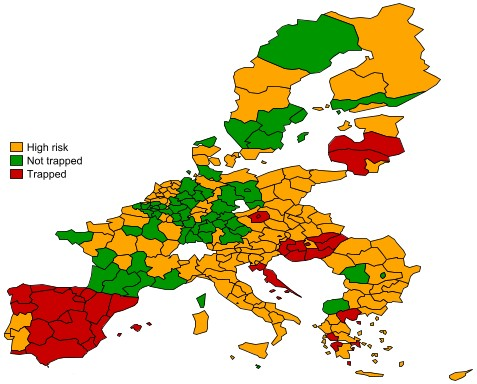
\includegraphics[width=.8\linewidth]{Figures/FDTR_2008-2015.jpg}
\end{figure}

\pagebreak
\clearpage

\begin{figure}%[htbp]
  \centering
 \caption{Classification of European Regions by Financial Development Trap Risk (2016–2021)}
 \vspace{-2mm}
 \caption*{\footnotesize This map displays the combined FDTR1 and FDTR2 classification for 226 European NUTS2 regions during the 2016--2021 period, which encompasses post-crisis recovery, ECB expansionary monetary policy, EU cohesion programmes, and the initial impact of the COVID-19 pandemic. Regions are classified as \textit{High Risk} (orange) when only one indicator exceeds its threshold, and \textit{Not trapped} (green) when neither indicator surpasses its respective risk threshold (FDTR1 $<$ 0.5 and FDTR2 $<$ 0.5). Notably, no regions were classified as \textit{Trapped} during this period, compared to 16.37\% in 2008--2015, indicating that no region simultaneously exhibited both recent deterioration (FDTR1 $>$ 0.75) and persistent structural slowdown (FDTR2 $>$ 1.5). During this period, 60.18\% of regions remained at high risk while 39.82\% were not trapped.}
  \label{fig:class1621}
  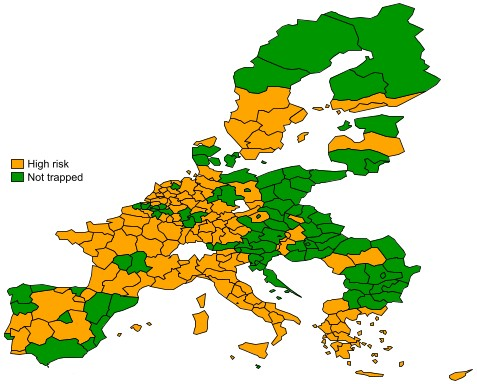
\includegraphics[width=.8\linewidth]{Figures/FDTR_2016-2021.jpg}
\end{figure}

\pagebreak
\clearpage



\begin{figure}%[htbp]
  \centering
 \caption{Spatial Distribution of Financial Development Trap Risk 1 (2008-2015)}
 \vspace{-2mm}
 \caption*{\footnotesize This map displays the spatial distribution of FDTR1 values for 226 European NUTS2 regions during the 2008--2015 period. FDTR1 measures the proportion of non-positive accelerations across six dimensions: two for each of the three indicators (GDP per capita, financial sector productivity, and financial sector employment rate)---one relative to the region's own past trajectory and one relative to the EU average. Values range from 0 (all accelerations positive) to 1 (no positive accelerations), with darker shades indicating higher entrapment risk.}
  \label{fig:fdtr10815}
  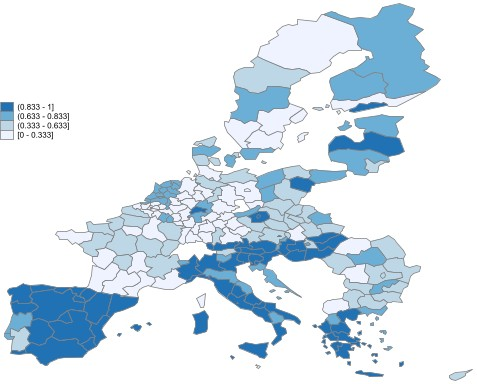
\includegraphics[width=.8\linewidth]{Figures/FDTR1_2008-2015.jpg}
\end{figure}

\pagebreak
\clearpage

\begin{figure}%[htbp]
  \centering
 \caption{Spatial Distribution of Financial Development Trap Risk 1 (2016-2021)}
 \vspace{-2mm}
 \caption*{\footnotesize This map displays the spatial distribution of FDTR1 values for 226 European NUTS2 regions during the 2016--2021 period. FDTR1 measures the proportion of non-positive accelerations across six dimensions: two for each of the three indicators (GDP per capita, financial sector productivity, and financial sector employment rate)---one relative to the region's own past trajectory and one relative to the EU average. Values range from 0 (all accelerations positive) to 1 (no positive accelerations), with darker shades indicating higher cyclical vulnerability.}
  \label{fig:fdtr11621}
  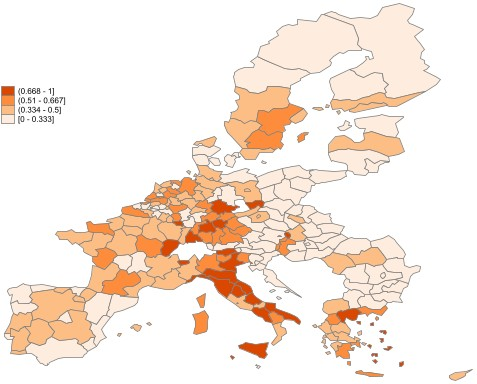
\includegraphics[width=.8\linewidth]{Figures/FDTR1_2016-2021.jpg}
\end{figure}







\end{document}




